\documentclass[a4paper, 12pt, diplomski]{etf}

\usepackage{cmsrb}
\usepackage[OT2,T1]{fontenc}

\usepackage[intlimits]{amsmath}
\usepackage{amsmath, amsfonts, amssymb, graphicx}
\usepackage{cite}
\usepackage{xcolor}
\usepackage[margin=1in]{geometry}


\usepackage[
    type={CC},
    modifier={by-sa},
    version={4.0},
]{doclicense}

%%%% XELATEX

\usepackage{fontspec}
\usepackage{indentfirst}
%\usepackage[margin = 0.5in]{geometry}
\usepackage{titletoc}
\usepackage[Symbolsmallscale]{upgreek}
\usepackage[serbian]{babel}
\usepackage{amsmath}
\usepackage{amssymb}
\usepackage{siunitx}
\usepackage{subcaption}
\usepackage{graphicx}
\usepackage{icomma}
\usepackage{cancel}
\usepackage{physics}
\usepackage{tikz}
\usepackage{environ}
\usepackage[thinc]{esdiff}
\everymath{\displaystyle}
\usepackage{listings}
\usepackage{url}
\usepackage{xcolor}
\usepackage{enumerate}
\usepackage[bottom]{footmisc}

%\usepackage{setspace}
%\doublespacing

\setcounter{tocdepth}{3}
\setcounter{secnumdepth}{3}

\definecolor{codegreen}{rgb}{0,0.6,0}
\definecolor{codegray}{rgb}{0.5,0.5,0.5}
\definecolor{codepurple}{rgb}{0.58,0,0.82}
\definecolor{backcolour}{rgb}{0.95,0.95,0.92}
\definecolor{pythonC0}{HTML}{1F77B4} 
\definecolor{pythonC1}{HTML}{FF7F0E} 

\lstdefinestyle{mystyle}{
    backgroundcolor=\color{backcolour},   
    commentstyle=\color{codegreen},
    keywordstyle=\color{magenta},
    numberstyle=\tiny\color{codegray},
    stringstyle=\color{codepurple},
    basicstyle=\ttfamily\footnotesize,
    breakatwhitespace=false,         
    breaklines=true,                 
    captionpos=b,                    
    keepspaces=true,                 
    numbers=left,                    
    numbersep=5pt,                  
    showspaces=false,                
    showstringspaces=false,
    showtabs=false,                  
    tabsize=2
}

\lstset{style=mystyle}

\usepackage{etoolbox}
\patchcmd{\thebibliography}{\chapter*}{\section*}{}{}

\addto{\captionsserbian}{%
  \renewcommand{\bibname}{Literatura}
}

\usepackage{accents}
%\newcommand{\ul}[1]{\underaccent{\bar}{#1}}
\newcommand{\ubar}[1]{\mkern3mu\underline{\mkern-3mu #1\mkern-3mu}\mkern3mu}

\usepackage{mathtools}
%\newcommand{\ubar}[1]{\mathrlap{\underline{\vphantom{#1}\hphantom{\textup{#1}}}}#1}

\righthyphenmin1
\lefthyphenmin1

\newcommand{\navod}[1]{„#1“}
\newcommand{\unit}[1]{\,{\rm #1}}
%\usepackage{mathptmx}
%\setmainfont{Times New Roman}'
\newcommand{\DS}{\displaystyle}
%\newcommand{\faz}[1]{\underbar{#1}}

\usepackage{accents}
\newcommand{\faz}[1]{\underaccent{\bar}{#1}}

%%%

%\title{
%Implementacija i postupak kalibracije skalarnog analizatora %mreža 
%u opsegu mikrotalasnih učestanosti 300\,MHz -- 3\,GHz
%}
%\author{Danilo Đokić}
%\indeks{2016/0116}
%\date{Septembar 2020.}
%\mentor{doc. dr Slobodan Savić}
%\predmet{}

\frenchspacing

\begin{document}

%\fontencoding{OT2}\selectfont

%\maketitle

\begin{center}
    {
    \Large
    \textsc{Univerzitet u Beogradu} \\
    \textsc{Elektrotehnički fakultet} \\
    \includegraphics[scale=.5]{fig/etf-logo-lat.jpg}
    
    \vfill
    
    \LARGE
    Implementacija i postupak kalibracije skalarnog
    analizatora mreža u opsegu mikrotalasnih učestanosti
    od $300\unit{MHz}$ do $3\unit{GHz}$
    } \\[2mm]
    {\large Diplomski rad}
    
    \vfill
    
    \large 
    
    \begin{minipage}{.49\textwidth}
    Mentor:     \\
    Dr Slobodan Savić, docent
    \end{minipage}
    \begin{minipage}{.49\textwidth}
    \begin{flushright}
    Kandidat: \\
    Danilo Đokić, 2016/0116
    \end{flushright}
    \end{minipage}

    
    \vfill
    
    Beograd, Septembar 2020.
\end{center}

\thispagestyle{empty}

\newpage

\tableofcontents

\begingroup
\let\clearpage\relax
\listoffigures
\endgroup

\newpage

%\begin{abstract}
%\end{abstract}

%\begin{keywords}
%\end{keywords}

%\tableofcontents
%\listoffigures
%\listoftables

\begin{abstract}

    Analizator mreža je jedan od osnovnih mernih instrumenata
    za rad u mikrotalasnom području učestanosti. U 
    ovom radu su uvedeni i objašnjeni osnovni 
    principi funkcije tog instrumenta. Realizovana
    su dva instrumenta radi ilustracije određenih 
    teorijskih rezultata.
    
    Rad je organizovan u pet odeljaka. U uvodu 
    su uvedeni opšti pojmovi koji se odnose 
    na Mikrotalasnu tehniku i merenja. U 
    odeljku „Karakterizacija mreža na mikrotalasnim
    učestanostima“ uveden je i definisan pojam 
    parametara rasejanja, kao i principi
    merenja. U odeljku
    „Analizator mreža“ je definisana osnovna struktura 
    instrumenta i njegove komponente, kao i parametri
    koji ih definišu. U istom poglavlju su navedeni
    dobijeni rezultati za kalibraciju senzora nivoa
    snage koji se koriste u ovom radu i opisana je 
    arhitektura mernog sistema sa strane upravljanja.
    U odeljku „Rezultati i diskusija“ su navedeni
    rezultati četiri ogleda koji imaju za cilj 
    demonstraciju rada projektovanog sistema kao i 
    ilustraciju ranije izvedenih teorijskih relacija.
    
    Premisa rada je da je moguće, imajući precizan
    referentni instrument, odgovarajućim postupkom
    kalibracije replicirati njegove ključne performanse
    na značajno pristupačnijem hardveru. U radu je opisana
    metodologija odabira komponenti koja se može proširiti i na drugačije radne zahteve. Implementirana
    je i biblioteka u programskom jeziku 
    \texttt{Python} koja komunicira sa uređajima u
    postavci, čime je korisniku ponuđen jednostavan 
    programski interfejs. \\[10mm]
    
    \doclicenseThis
    
    \vspace{1mm}
    
    Za slaganje najvećeg broja slika u ovom radu korišćena
    je \texttt{Xcircuit} biblioteka
    dostupna na \url{http://tnt.etf.rs/~dgrujic/xcircuit/},
    izmenjena i proširena za potrebe rada.
    \\[1mm]
    
    Online repozitorijum sa izvornim kodom dosupan je
    na \url{https://github.com/djokicd/ArduinoSNA}.
\end{abstract}

\newpage

\section{Uvod}
\subsection{Mikrotalasna tehnika}
Na dovoljno niskim učestanostima kola i komponente se mogu predstaviti modelom mreža sa koncentrisanim 
parametrima. Takva kola opisuju električne elemente u fizički ograničenom delu prostora između kojih nema elektromagnetske sprege, osim preko kondukcionih veza provodnicima za povezivanje, koji se
modeluju kao idealni kratki spojevi. 
U takvim kolima se zanemaruju i razni drugi 
efekti, kao što su efekti prostiranja, a kod 
idealnih elemenata (otpornik, kalem i 
kondenzator), smatra se da je izražen samo 
jedan elektromagnetski fenomen (Džulovi gubici, indukovana elektromotorna sila, odnosno nagomilavanje naelektrisanja).
Ovakva kola su opisana 
Kirhofovim zakonima, kao i stujno--naponskim karakteristikama
pojedinih elemenata koje u opštem slučaju mogu biti 
nelinearne i nejednoznačne. Električna merenja na ovim učestanostima 
se, pre svega, usredsređuju na direktna merenja napona i struja.

Mikrotalasna tehnika je oblast elektrotehnike koja se bavi projektovanjem komponenti
i kola u opsegu učestanosti od 300\,MHz do 300\,GHz. Na ovim učestanostima
efekti prostiranja dolaze do izražaja, tako da talasna priroda elektromagnetskih pojava dominira,
a Kirhofovi zakoni praktično prestaju da važe. Adekvatan opis ovakvih pojava se može izvesti isključivo 
uz uvažavanje ovih efekata i neposrednu analizu strukture elektromagnetskog polja Maksvelovim 
jedančinama u opštem slučaju. 
Procena validnosti pretpostavke o kolu sa raspodeljenim parametrima se može načinti poređenjem sa talasnom dužinom elektromagnetskog talasa koji se prostire u slobodnom prostoru sa najvećom dimenzijom kola.
Brzina prostiranja elektromagnetskog talasa u vakuumu je približno $c_0 \approx 300\unit{\dfrac{mm}{ns}}$
pa je talasna dužina 
$\DS \uplambda_0 = \frac{c_0}{f} \approx \frac{300
\,{\unit{mm/ns}}}{f}$.
Ukoliko je talasna dužina mnogo veća od dimenzije uređaja onda se efekti prostiranja praktično mogu zanemariti,
a uređaj se, u načelu, može analizirati kao kolo sa koncentrisanim parametrima. U suprotnom, efekti
prostiranja su izraženi, a kolo se mora tretirati kao kolo sa raspodeljenim parametrima. U okviru mikrotalasnih učestanosti ove talasne dužine su u
 opsegu od $1\unit{mm}$ do $1\unit{m}$, što su ujedno i najčešće dimenzije 
 električnih naprava. Posebno, efekti prostiranja su izraženi u pojedinim
 sistemima na niskim učestanostima koji su relativno velikih dimenzija, 
 kao 
 što su na primer 
% NOTE::
% lambda = c0/50 Hz = 6000 km
% EES u Evropi je lambda (u vakuumu)
elektroenergetski vodovi.
Suprotno, efekti prostiranja mogu 
 da ne budu izraženi i na visokim učestanostima, reda $10\unit{GHz}$, na 
 primer u integrisanim kolima koja su malih dimenzija, reda $100\unit{\upmu m}$.
 \cite{djordjevic-mw, pozar}

\subsection{Mikrotalasna merenja}
Klasična električna merenja u elektronici se izvode 
instrumentima poput osciloskopa, strujnih transformatora ili unimera. U opštem slučaju, za merenje napona je potrebno da merni instrument ostvari kvalitetnu otvorenu vezu (veliku ulaznu impedansu) koja paralelnim vezivanjem na ispitivani element
ne remeti značajno topologiju kola; dok je za merenje struja potrebno da merni instrument ostvari
kvalitetan kratak spoj (malu ulaznu impedansu) koja rednim vezivanjem na ispitivani element takođe ne
remeti topologiju kola. Kolike konkretno treba da budu te impedanse zavisi od prilika u kolu, 
% NOTE:: 
% Komentar je bio: "od velicine koja se meri"
% Konkretno mislim da merni opseg unimera 
% gde je mA - Ohm, ua - kOhm, na - MOhm
ali i od odabira mernih opsega odgovarajućih instrumenata.
Ostvarivanje takvih kratkih spojeva i otvorenih veza je, u načelu, jednostavno postići
u veoma širikom opsegu niskih učestanosti, na primer
DC -- 1\,MHz. Takva merenja uključuju linearne i nelinearne mreže, kao i jednoznačne i 
nejednoznačne mreže (npr. merenje histerezisa) \cite{Peja1}. Pri visokim učestanostima (VF), elektronske komponente se mogu dodatno opisati i paraznitnim elementima koji modeluju sekundarne fizičke efekte
u komponentama, kućištima uređaja ili same veze između uređaja. 
Na taj način se, kroz ekvivalentne modele, proširuje opseg učestanosti u kome se i dalje zadovoljavajuće tačno mogu primenjivati 
Kirhofovi
zakoni i klasična teorija električnih kola.
Ovaj pristup omogućuje da se
karakterišu i kola na znatno višim učestanostima.
Ipak, na dovoljno visokim učestanostima, model sa
koncentrisanim parametrima prestaje da važi, budući da upravo pretpostavke iz kojih su izvedeni Kirhofovi zakoni prestaju da važe.
\cite{mwmeas}

\section[Karakterizacija mreža na mikrotalasnim  učestanostima]{Karakterizacija mreža na mikrotalasnim \\ učestanostima}
\subsection{Prostiranje talasa na vodovima}
Za vodove na visokim učestanostima je neophodna jasna 
definicija geometrije, što omogućava konkretan opis u elektromagnetskom
smislu.
Pokazuje se da na cilindričnom vodu konstantnog poprečnog preseka sa homogenim dielektrikom,
u prostoperiodičnom režimu, 
mogu da se
prostiru dva transverzalna elektromagnetska talasa u suprotnim smerovima\footnote{
Strogo govoreći, prostiranje transverzalnih elektromagnetskih talasa duž vodova sa nehomogenim
dielektrikom nije moguće. Ipak, i u vodovima sa nehomogenim dielektrikom, na nižim mikrotalasnim 
učestanostima mogu da se prostiru tzv. kvazi-TEM talasi, čije su karakteristike praktično iste kao
one kod TEM talasa, pa se te analize ekvivalentiraju. Budući da su takvi vodovi relativno česti u praksi,
npr. mikrotrakasti vod, te da ova aproksimacija ne pravi velike greške, u daljem tekstu nećemo razlikovati kvazi-TEM talas od TEM talasa.
} koji su opisani svojim
kompleksnim intenzitetima,
kao na slici \ref{load}.
%
%
\begin{figure}[b]
    \centering
    \includegraphics{fig/prijemnik.pdf}
    \caption{Vod zatvoren linearnim prijemnikom.
    }
    \label{load}
\end{figure}
%
Argumenti kompleksnih intenziteta talasa odgovaraju 
argumentima kompleksnih predstavnika transverzalnog električnog polja,
dok su moduli jednaki korenu
srednje snage progresivnog talasa u datom smeru 
($|\faz a| = \sqrt{P_{\rm i}}$, 
$|\faz b| = \sqrt{P_{\rm r}}$).
Ukoliko se vod zatvori lineranim prijemnikom, zbog posledica graničnog uslova talasne 
jednačine napona na vodu, uspostavlja se veza između ova dva talasa (Slika \ref{load}). U odnosu na 
prijemnik, talasi se nazivaju incidentnim i reflektovanim, odnsno $a$ i $b$ prema slici. Odnos kompleksnih intenziteta incidentnog
i reflektovanog talasa se naziva kompleksnim 
koeficijentom refleksije prijemnika i određen je izrazom
\begin{equation}
    \faz \Upgamma = \frac {\faz b}{\faz a} 
    = \frac{ \faz Z_{\rm p} - \faz Z_{\rm c}  }
    {\faz Z_{\rm p} + \faz Z_{\rm c}}, \label{eq:gamma}
\end{equation}
gde su $\faz Z_{\rm p}$ kompleksna impedansa prijemnika
i $\faz Z_{\rm c}$ primarni parametar voda i predstavlja 
njegovu karakterističnu impedansu. Napomenimo da je karakteristična impedansa voda sa gubicima u opštem slučaju kompleksna veličina.
Ipak, ukoliko se gubici mogu zanemariti, karakteristična impedansa je praktično
realna veličina, ${\bf I}{\rm m}\{
\faz Z_{\rm c}\} 
\approx 0$, pa ćemo zbog toga u nastavku smatrati da je $Z_{\rm c}$ čisto realno.
Naročito, navedimo da je impedansa $\faz Z_{\rm 2}$, u preseku (2), mreže sa slike 
\ref{load} određena izrazom
\begin{equation}
    \faz Z_{\rm 2} = \frac
    { \faz Z_{\rm p} + {\rm j} Z_{\rm c} \tan(\upbeta L) }  
    {  Z_{\rm c} + {\rm j}\faz Z_{\rm p} \tan(\upbeta L) },
    \label{eq:zin}
\end{equation}
gde su $\upbeta = \dfrac{\upomega}{c}$ 
i $L$
fazni koeficijent i fizička dužina voda, respektivno.
%
Posebno, prijemnik za koji je, prema izrazu
\eqref{eq:gamma},  $\faz Z_{\rm p} = Z_{\rm c}$,
nema refleksiju ($\faz \Upgamma = 0$) 
 i naziva se prilagođenjem. 
Naglasimo još da su merenja i analiza nelinarnih 
elemenata u mikrotalasnim kolima značajno složeniji
nego na niskim učestanostima i neće biti 
tema ovog rada.

\subsection{Parametri rasejanja}
Prijemnik opisan u prethodnoj tački se može 
smatrati za mrežu sa jednim pristupom. U opštem 
slučaju, mikrotalasne mreže mogu imati i više pristupa,
u kom slučaju se koncept koeficijenta refleksije 
može uopštiti. Na sličan način na koji se definišu
impedansni ili admitansni 
parametri za napone i struje na pristupima,
mogu se definisati i parametri rasejanja za 
intenzitete talasa na pristupima. Posmatrajmo 
proizvoljnu linearnu 
mrežu, bez generatora, sa $n$ pristupa prikazanu na slici 
\ref{fig:nport} i usvojimo skup nominalnih 
impedansi\footnote{
Nominalnim impedansama se može pripisati i 
fizički smisao. 
Nominalne impedanse se mogu shvatiti i kao karakteristične impedanse vodova za koje se očekuje da će se koristiti za povezivanje posmatane mreže u ostatak kola. U tom slučaju, analiza i merenje mreže su značajno jednostavniji nego ako bi se definisao jedan skup nominalnih impedansi, a za merenje koristio drugačiji skup karakterističnih impedansi vodova za povezivanje.
} $Z_{\rm 01}, Z_{\rm 02}, \ldots, Z_{0n}$.
%
\begin{figure}[b!]
    \centering
    \includegraphics{fig/nport.pdf}
    \caption{Uz definiciju parametara rasejanja.
    }
    \label{fig:nport}
\end{figure}
%
Budući da je mreža linearna, veza između vektora $[\faz {\bf b}] 
= [\faz b_1\ \faz b_2\ \cdots \faz b_n]^{\rm T}$
i $[\faz {\bf a}] = [
\faz a_1\ \faz a_2\ \cdots \faz a_n]^{\rm T}$ je linearna i može se raspisati matrično kao

\begin{equation}
[\faz{\bf b}] = [\faz{\bf S}] [\faz{\bf a}] 
\quad \quad \text{gde je} \quad \quad
[\faz {\bf S}]
=
\begin{bmatrix}
\faz s_{11} & \faz s_{12} & \cdots & \faz s_{1n}\\ 
\faz s_{21} & \faz s_{22} & \cdots & \faz s_{2n} \\
\vdots & \vdots & \ddots & \vdots \\ 
\faz s_{n1} & \faz s_{n2} & \cdots & \faz s_{nn}
\end{bmatrix}, 
    \label{eq:spar}
\end{equation}
%
gde su $\faz s_{ij}$ odgovarajući parametri rasejanja.
Parametri rasejanja zavise od nomimalnih impedansi,
tako da je linearna mreža bez nezavisnih
generatora opisana u potpunosti 
matricom rasejanja i odabirom nominalnih 
impedansi. U praksi je najčešće da su sve 
nominalne impedanse jednake  $Z_{\rm 01} = Z_{\rm 02} = \ldots = Z_{0n} = Z_0$, a u mikrotalasnoj tehnici je 
ustaljena standardna vrednost nominalne impedanse 
od $Z_0 = 50\unit{\Upomega}$, mada ima i drugih standarda.

Postupak merenja parametara 
rasejanja
se izvodi koristeći se obrazloženim principom prilagođenja pristupa $(i)$ da bi se
anulirao odgovarajući incidentni talas $a_i$
na svim prilagođenim pristupima. Ovaj postupak je
ilustrovan na slici \ref{fig:nport_measure}. Zamenom 
$\faz a_j = 0$ za $j \neq i$ i 
$1 \leq j \leq n$
u izraz \eqref{eq:spar} dobijaju se veze
\begin{equation}
\begin{bmatrix}
\faz b_1\\ 
\faz b_2\\ 
\vdots \\ 
\faz b_i \\
\vdots \\
\faz b_n
\end{bmatrix}
=
\begin{bmatrix}
\faz s_{11} & \faz s_{12} & \cdots & \faz s_{1n}\\ 
\faz s_{21} & \faz s_{22} & \cdots & \faz s_{2n} \\
\vdots & \vdots & \ddots & \vdots \\ 
\faz s_{n1} & \faz s_{n2} & \cdots & \faz s_{nn}
\end{bmatrix} 
\cdot
\begin{bmatrix}
0\\ 
0\\ 
\vdots \\ 
\faz a_i \\
\vdots \\
0
\end{bmatrix}
\Rightarrow
\left\{\begin{matrix}
\faz b_1 = \faz s_{1i} \faz a_i \\
\faz b_2 = \faz s_{2i} \faz a_i \\
\vdots \\
\faz b_i = \faz s_{ii} \faz a_i \\
\vdots \\
\faz b_n = \faz s_{ni} \faz a_i \\
\end{matrix}\right. .
\label{eq:spar_meas}
\end{equation}
%
\begin{figure}[b!]
    \centering
    \includegraphics{fig/nport_measure.pdf}
    \caption{Uz merenje parametara rasejanja.}
    \label{fig:nport_measure}
\end{figure}
%
% NOTE::
% Razdvojio sam ove dve grupe parametara zato
% što je način na koji se mere praktično
% različit. 
Na osnovu dobijenog rezultata parametri $\faz s_{ki} = \frac{\faz b_k}{\faz a_i}$ $(k\neq i)$ predstavljaju parametre prenosa kroz mrežu od $i$-tog
ka $k$-tom pristupu kada su svi ostali pristupi zatvoreni svojim nominalnim impedansama. 
Prenetu snagu (na osnovu koje je moguće izračunati intenzitet talasa $\faz{b}_k$) talasa je potrebno 
premeriti u okviru prijemnika na $k$-tom pristupu, odnosno, 
taj prijemnik bi trebalo da bude dobro prilagođen detektor
snage\footnote{
Ovi detektori snage mogu biti utemeljeni na različitim 
fizičkim principima. Neki mere zagrevanje na račun disipirane snage
u vidu \textsc{Joule}ovih gubitaka, dok su neki zasnovani 
na aktivnim logaritamskim detektorima. Razlikuju se 
prema
osnovnim karakteristikama, opsegu ulazne snage i preciznosti.
}. Za parametar  $\faz s_{ii} = \frac{\faz b_i}{\faz a_i}$ je jasno,
na osnovu izraza \eqref{eq:gamma}, 
da predstavlja koeficijent 
refleksije na $i$-tom pristupu i potrebno ga je meriti razdvajanjem incidentnog 
i reflektovanog talasa, o čemu će biti reči kasnije.
%
%

Prokomentarišimo još da je karakterizacija mikrotalasnih
mreža jednostavnija prema parametrima rasejanja i zbog 
toga što je tehnička realizacija širokopojasnih 
prilagođenja jednostavnija nego kratkih spojeva i
otvorenih veza. 
Dodatno, 
nekada je nemoguće napraviti kvalitetan kratak spoj ili otvorenu vezu. Na primer, kratak
spoj u vidu  
vije na štampanoj ploči, ukoliko je supstrat
dovoljno debeo, ili otvoreni kraj talasovoda
koji onda i zrači tokom merenja. 
Takođe, kratak spoj i otvorena veza odgovaraju
prijemnicima maksimalnog koeficijenta 
refleksije što može da poremeti rad 
ispitivanih aktivnih naprava kao što su,
na primer, pojačavači.


\section{Analizator mreža}
\begin{figure}[ht!]
    \centering
    \includegraphics{fig/na.pdf}
    \caption{Uz merenje analizatorom mreža.}
    \label{fig:na}
\end{figure}
Instrument koji može da meri karakteristike linearnih
mikrotalasnih mreža se naziva analizatorom 
mreža. Najčešće, minimalna funkcionalnost ovih instumenata
uključuje automatsko merenje parametara rasejanja barem 
dvopristupnih mreža u nekom opsegu učestanosti,
mada može uključivati i složeni sistem obrade 
dobijenih rezultata. 
Analizator treba da pobuđuje mrežu i da na odgovarajući  način prati njen odziv. Mada je 
principska šema za merenje parametara rasejanja,
ilustrovana na slici \ref{fig:nport_measure},
jednostavna, tehnički
detalji ovakvih realizacija, kao i nesavršenosti
komponenti, iziskuju 
složenije
topologije u cilju izvođenja i optimizacije merenja. Šema
povezivanja instrumenta treba da bude jednostavna i prikazana je na slici 
\ref{fig:na}.

U pogledu složenosti merenja parametara rasejanja 
analizatori mreža se načelno dele na 
\begin{itemize}
    \item Vektorske analizatore mreža 
    (eng. \textit{Vector Network Analyzer} -- VNA) koji
    imaju mogućnost 
    da mere i modul i argument $s$-parametara,
    time u potpunosti opisujući mrežu; i
    \item Skalarne analizatore mreža
    (eng. \textit{Scalar Network Analyzer} --
    SNA) koji mogu da mere samo 
    modul $s$-parametara, čime se mreža 
    delimično opisuje.
\end{itemize}
Iako vektorski analizatori u potpunosti
opisuju mrežu, njihova složenost, a samim tim i cena, je višestruko
veća od skalarnih. Ipak, skalarni 
analizatori su često dovoljni za karakterizaciju
gotovih, najčešće jednopristupnih ili dvopristupnih sistema
kao što su antene, filtri ili pojačavači. U tom pogledu se
definišu naročiti tehnički nazivi modula parametara 
rasejanja dvopristupnih mreža, i to
\begin{enumerate}
    \item Povratni gubici na ulaznom 
    pristupu (eng. \textit{Input Return Loss}), 
    $${\rm IRL} = - 20 \log_{10}|\faz s_{11}|\unit{[dB]};$$ 
    \item Povratni gubici na izlaznom 
    pristupu (eng. \textit{Output Return Loss}), 
    $${\rm ORL} = - 20 \log_{10}|\faz s_{22}|\unit{[dB]};$$
    \item Uneto slabljenje (eng. \textit{Insertion loss}), 
    $${\rm IL} = - 20 \log_{10}|\faz s_{21}|\unit{[dB]},$$ za mreže sa gubicima u 
    prenosu; i
    \item Pojačanje snage (eng. \textit{Gain}), 
    $$G = 20 \log_{10}|\faz s_{21}|\unit{[dB]},$$ za mreže koje ostvaruju pojačanje.
\end{enumerate}
\subsection{Komponente SNA}
Blok dijagram osnovnog skalarnog analizatora mreža je prikazan
na slici \ref{fig:sna_block}. Na slici su prikazani
pobudni generator, ispitivani uređaj 
(eng. \textit{Device Under Test} - DUT), 
usmereni sprežnjak (obeležen sa DC)
i tri detektora nivoa snage $p_{\rm E}$,
$p_{\rm R}$ i $p_{\rm T}$. 
% NOTE::
% Detektori mere nivo snage znači mala slova? 
%
\begin{figure}[b!]
    \centering
    \includegraphics{fig/sna_block_simple.pdf}
    \caption{Topologija skalarnog analizatora mreža.}
    \label{fig:sna_block}
\end{figure}
%
Zadatak 
usmerenog sprežnjaka je da razdvoji 
incidentni i reflektovani talas na 
pristupu (1) ispitivanog uređaja, dok 
detektori snage mere incidentnu snagu i
treba da budu dobro prilagođeni. Merenja 
nivoa
snaga $p_{\rm E}$, $p_{\rm R}$ i $p_{\rm T}$ predstavljaju:
 jedinični/referentni nivo snage, nivo
 reflektovane snage i nivo 
 transmitovane snage, respektivno. Na osnovu rezultata merenja ovih snaga se ustanovljavaju parametri rasejanja prema\footnote{
Jedinica dBm je decibel u odnosu na milivat i predstavlja
logaritamsku meru nivoa snage definisanu sa 
$p = 10 \log_{10} 
\left( \dfrac{P}{1\unit{mW}} \right) \unit{dBm}$
}
\begin{equation}
   |\faz s_{11}| = \sqrt{ \dfrac{P_{\rm R}}{P_{\rm E}} } \Rightarrow
    s_{11}^{[\rm dB]}
    = p_{\rm R}^{[\rm dBm]} - p_{\rm E}^{[\rm dBm]},
    \quad
    |\faz s_{21}| = \sqrt{ \dfrac{P_{\rm T}}{P_{\rm E}} } \Rightarrow
    s_{21}^{[\rm dB]}
    = p_{\rm T}^{[\rm dBm]} - p_{\rm E}^{[\rm dBm]}
    \label{eq:s11s212}
\end{equation}
%
Ova konkretna topologija omogućava merenje povratnih gubitaka i 
unetog slabljenja, tako da je za merenje sva četiri parametra
rasejanja za dvoportne mreže 
neophodno
izvršiti merenje za dve topologije, u kojima se 
razlikuje pozicija pobudnog generatora i mesta 
gde se mere nivoi snaga.
%
Ovaj problem principski nije teško rešiti uvođenjem dva
poluprovodnička preklopnika, ali ćemo se u ovom radu,
radi jednostavnosti, zadržati na 
ovoj topologiji.
U nastavku će detaljno biti opisane karakteristike i ograničenja
ovih komponenti koje utiču na rad sistema. 

\subsubsection{Pobudni generator}
Pobudni generator treba da bude prilagođeni generator koji pobuđuje
incidentan talas na jednoj učestnosti za koju je konfigurisan.
Blok simbol generatora je prikazan
na slici \ref{fig:vsymb}. Generator treba 
da obezbedi programsko podešavanje učestanosti, dok nivo signala treba 
da bude dovoljno veliki tako da snaga koja stiže do detektora bude 
dovoljno velika da premašuje prag osetljivosti. Ukoliko je dodatno potrebno regulisati i izlaz generatora prema snazi,
moguće je postaviti i digitalni atenuator, a onda u povratnoj sprezi sa odgovarajućim senzorom 
podešavati izlaznu snagu
(eng. \textit{Automatic Level Control} -- ALC). 
U pogledu intenziteta talasa, ponašanje generatora je opisano 
izrazom
\begin{equation}
    \faz b = \faz b_{\rm g} + 
    \faz \Upgamma_{\rm g} \faz a.
\end{equation}

Glavne karakteristike
generatora koje ograničavaju njegove
performanse su neprilagođenje i
fazni šum.
Neprilagođenje ograničava dinamički opseg, dok fazmi šum, 
koji predstavlja kratkoročnu nestabilnost učestanosti, predstavlja 
ograničenje u pogledu rezolucije po učestanosti. 
U ovom radu se neće detaljno
razmatrati uticaji pobudnog generatora i smatraće 
se da je on savršen.
%
\begin{figure}[ht!]
        \centering
        \includegraphics[scale = 1]
        {fig/vgen_symbol.pdf}
        \caption{Oznaka pobudnog generatora.}
        \label{fig:vsymb}
\end{figure}

\subsubsection{Usmereni sprežnjak \label{ss:dc}}
Usmereni sprežnjak (eng. \textit{Directional Coupler} -- DC) je 
pasivna mreža sa četiri pristupa, čija je uloga da razdvoji incidentni
i reflektovani talas na vodu.
Njegova oznaka je prikazana na slici \ref{fig:dc}.
Usmereni sprežnjaci pogodni za primenu u 
analizatorima mreža imaju takvu karakteristiku
da su njihovim priključenjem na liniju gde se 
mere snage incidentnog i reflektovanog talasa 
praktično „nevidljivi“ u ostatku kola. 
To podrazumeva da su
uloge pristupa određene prema:
\begin{enumerate}
    \item Ulazni pristup --- Talas doveden na ulazni pristup se u 
    najvećoj meri prenosi do izlazanog pristupa;
    \item Izlazni pristup --- Talas doveden na izlazni pristup se 
    u najvećoj meri prenosi do ulaznog pristupa;
    \item Izolovani pristup --- Do ovog pristupa \textbf{ne} dolazi talas
    kojim je pobuđen ulazni pristup, ali dolazi deo 
    talasa koji se reflektuje na
    izlaznom pristupu;
    \item Spregnuti pristup --- Do ovog pristupa dolazi talas
    kojim je pobuđen ulazni pristup, ali \textbf{ne} dolazi deo talasa koji se reflektuje na
    izlaznom pristupu.
\end{enumerate}
%
\begin{figure}[t!]
    \centering
    \includegraphics{fig/dc.pdf}
    \caption{Oznaka usmerenog sprežnjaka.}
    \label{fig:dc}
\end{figure}
%
Parametri rasejanja realnog usmerenog sprežnjaka, pod pretpostavkom 
da su pristupi savršeno prilagođeni, 
opisani su parametrima $\faz c$ (eng. \textit{coupling}) i $\faz i$ (eng. 
\textit{isolation}) koji kvantizuju u kojoj meri dolazi
do navedenih prenosa kao
\begin{equation}
    [{\bf \faz S}] = 
    \begin{bmatrix}
    0 & \faz E & \faz i & \faz c\\ 
    \faz E & 0 & \faz c & \faz i \\
    \faz i & \faz c & 0 & \faz E \\
    \faz c & \faz i & \faz E & 0 \\
    \end{bmatrix}. 
\end{equation}
%
Kako je u 
usmerenim sprežnjacima koji se koriste u okviru analizatora mreža
$1 \gg |\faz c| \gg |\faz i|$, to je 
$|\faz E| \approx 1$, na osnovu osobine da je $s$-matrica pasivne mreže bez gubitaka ortonormalna. 
Odnos modula parametara 
sprege i izolacije se naziva direktivnošću usmerenog
sprežnjaka i definiše se kao $D = \dfrac{|\faz c|}{|\faz i|}$.


%Parametri sprege i izolacije su čestno i manji od 
%$-20\unit{dB}$ pa je gubitak snage pri prolasku kroz sprežnjak manji
%od 1\%. Naročito je potrebno primetiti da su, zbog simetrije, 
%pristupi (3) i (4) dobro spregnuti tako da je za poterbe 
%merenja spregnutog signala sa pristupa (1) na pristupu (4) neophodno kvalitetno prilagoditi pristup (3).

Osnovna nesavršenost usmerenog sprežnjaka
je uzrokovana prenosom talasa 
sa izolovanog porta ($i\neq 0$).
Za određivanje uticaja te nesavršenosti 
posmatrajmo deo kola prikazan na slici
\ref{fig:dc_imp}, gde su detektori 
i deo kola desno od ispitivanog uređaja
zamenjeni prilagođenjima, a pobudni 
generator je savršeno prilagođen.
%
\begin{figure}[t!]
    \centering
    \includegraphics{fig/dc_imperf.pdf}
    \caption{Uz nesavršenost usmerenog
    sprežnjaka.}
    \label{fig:dc_imp}
\end{figure}
%
Neka su 
$a_1$ i $a_2$
intenziteti incidentnih talasa na pristupima (1) i (2) 
redom\footnote{
U ovoj tački, i u nastavku rada, ispraćena je konvencija
da su moduli kompleksnih veličina obeleženi 
bez podvlačenja, odnosno, 
$z = |\faz z|, z \in \mathbb C$.
}.
Tada su granice za 
intenzitete talasa koji dolaze do pristupa (3) i 
(4) određeni izrazima\footnote{
Znakom „$\pm$“ se označava uticaj
izolovanog signala koji je mali i koji se u dva granična slučaja
sabira i oduzima po intenzitetu. Ekvivalentno je 
$a - b \leq |\faz a + \faz b| \leq a + b$, za $|\faz b| < |\faz a|$.
}
$b_3 = ca_2 \pm ia_1$ i $b_4 = ca_1 \pm ia_2$.
Uzevši u obzir 
topologiju sa slike \ref{fig:sna_block}, zaključujemo da su 
$a_{\rm R} = b_3$ i $a_{\rm E} = b_4$,
odakle se, imajući u 
vidu izraz \eqref{eq:s11s212}, ima rezultat merenja
$ s_{\rm 11}^{\rm (m)} = \dfrac{a_{\rm R}}{a_{\rm E}} = 
\dfrac{ ca_2 \pm ia_1}{ ca_1 \pm ia_2}$. Primetimo dodatno 
da su $a_2 = E s_{11}^{\rm (DUT)} a_1 \approx s_{\rm 11}^{\rm (DUT)} a_1 $ i 
$
    ca_1 \gg ia_2
    \label{eq:ca1ia2}
$, odakle se ima
\begin{equation}
    s_{\rm 11}^{\rm (m)} = 
\dfrac{ ca_2 \pm ia_1}{ ca_1 \pm ia_2}
\approx 
\dfrac{ c s_{\rm 11}^{\rm (DUT)} a_1 \pm ia_1}{ ca_1} 
= s_{\rm 11}^{\rm (DUT)} \pm \dfrac{i}{c},
\label{eq:ioverc}
\end{equation}
odakle sledi da je granica apsolutne greške
merenja određena direktivnošću:
\begin{equation}
\Delta s_{\rm 11} = \frac{i}{c} = \dfrac 1D.
\end{equation}

\subsubsection{Detektor snage \label{ss:detektor}}
%
%
\begin{figure}[t!]
    \centering
    \includegraphics{fig/umatch_rfd.pdf}
    \caption{Uz uticaj neprilagođenja detektora.}
    \label{fig:umatch_rfd}
\end{figure}
%
\begin{figure}[b!]
    \hfill
    \begin{subfigure}[b]{0.39\textwidth}
        \centering
        \includegraphics[scale=0.83]{fig/rfd.pdf}
        \caption{Oznaka detektora snage.}
        \label{fig:rfd}
    \end{subfigure}
    %
    \hfill
    %
    \begin{subfigure}[b]{0.59\textwidth}
        \centering
        \includegraphics[scale=0.83]{fig/rfd_att.pdf}
        \caption{Prilagođenje atenuatorom.}
        \label{fig:rfd_att}
    \end{subfigure}
    %
    \hfill
    \caption{Uz detektor snage.}
\end{figure}
%
Detektor se u kolu ponaša kao linearni prijemnik čiji 
koeficijent refleksije 
može da zavisi od učestanosti, 
$\faz \Upgamma_{\rm D} = \faz \Upgamma_{\rm D} (\upomega)$. 
Detektor generiše stalni napon koji je određen primljenom snagom prema njegovoj
statičkoj karakteristici prenosa koja može biti i
nelinearna. 
Šematski simbol detektora je prikazan na slici 
\ref{fig:rfd}. 

Osnovna nesavršenost detektora ogleda se u njegovom 
neprilagođenju. Ukoliko je refleksija na njemu mala, onda se može
smatrati da se jednom reflektovani talas praktično ne vraća do 
detektora. Budući da senzor meri primljenu snagu, pod ovom pretpostavkom se može uspostaviti veza između incidentne snage
$P_{\rm i}$ i izmerene snage $P_{\rm D}$ kao
\begin{equation}
    P_{\rm i} = \dfrac{P_{\rm D}}{1 - |\faz \Upgamma|^2},
    \label{eq:corP}
\end{equation}
Sekundarna nesavršenost detektora jeste ograničenje mernog opsega nivoa 
snaga. Osetljivost senzora je određena minimalnim nivoom snage koju senzor pouzdano može da meri $p_{{\rm D,\, min0}}$.

Uticaj neprilagođenja detektora se može ustanoviti
postupkom analognim onome
izvedenom u prethodnoj tački. Razmotramo deo kola sa slike
\ref{fig:umatch_rfd}.
%
Za intenzitete incidentnih talasa detektora, ponovno usvojivši
$a_2 \approx s_{11}^{\rm (DUT)} a_1$, mogu se pisati
veze
\begin{equation}
    \begin{array}{c}
         a_{\rm R} = cs_{11}^{\rm (DUT)}a_1 \pm ia_1 + \Upgamma_{\rm D} a_{\rm E},  \\
         a_{\rm E} = ca_1 \pm is_{11}^{\rm (DUT)}a_1 + \Upgamma_{\rm D} a_{\rm R}.
    \end{array}
\end{equation}
Rešavanjem ovog sistema jednačina po $a_{\rm R}$ i $a_{\rm E}$ se može odrediti veza\footnote{
Znak „$\pm$“ treba tretirati na isti način kao u pređašnjem izvođenju
}
\begin{equation}
\dfrac{a_{\rm R}}{a_{\rm E}} = 
\dfrac{ \pm i(1 + s_{11}^{\rm (DUT)} \Upgamma_{\rm D}) + c(s_{11}^{\rm (DUT)} + \Upgamma_{\rm D})}
      { c(1 + s_{11}^{\rm (DUT)} \Upgamma_{\rm D}) \pm i(s_{11}^{\rm (DUT)} + \Upgamma_{\rm D}) } 
      \approx \dfrac{s_{11}^{\rm (DUT)} + \Upgamma_{\rm D}}{1 + s_{11}^{\rm (DUT)} \Upgamma_{\rm D}} \pm \dfrac 1D.
\end{equation}
Na osnovu ovog izraza, greška merenja je 
$\Updelta s_{11} = 
\dfrac{s_{11}^{\rm (DUT)} + \Upgamma_{\rm D}}{1 + s_{11}^{\rm (DUT)} \Upgamma_{\rm D}} \pm \dfrac 1D - s_{11}^{\rm (DUT)}
$, sređivanjem se dobija 
$
\Updelta s_{11} = 
\Upgamma_{\rm D} 
\dfrac{1 -  s_{11}^{\rm (DUT)} }{1 + \Upgamma_{\rm D}
 s_{11}^{\rm (DUT) }
}
\pm \dfrac 1D
$.
U najgorem slučaju
($ s_{11}^{\rm (DUT)} = 0$), nalazi se
granica greške merenja je $\Delta s_{11} = \dfrac 1D + \Upgamma_{\rm D}$, odakle se zaključuje da 
prilagođenje detektora treba da bude istog reda veličine kao direktivnost usmerenog sprežnjaka, inače direktivnost 
ima ograničavajući uticaj, a dalja poboljašanja prilagođenja neće imati značajan doprinos. 

Prilagođenje detektora se može pobošljati
povezivanjem atenuatora kao na slici \ref{fig:rfd_att}. 
Pokazuje se da se na ovaj način prilagođenje poboljšava za 
dvostruko slabljenje atenuatora (izraženo u decibelima),
\begin{equation}
    \Upgamma_{\rm D}'^{\rm [dB]}= \Upgamma_{\rm D}^{\rm [dB]} - 2A^{\rm [dB]}.
\end{equation}
Ovakvo prilagođenje je pogodno za ovakvu primenu pre svega zbog 
njegove širikopojanosti. Ipak, budući da ono unosi gubitke, minimalna snaga
koju detektor može da izmeri postaje veća. Zbog toga ovakvo prilagođenje 
predstavlja kompromis između dinamičkog opsega i efektivne osetljivosti 
detektora. Optimalno prilagođenje je na osnovu pređašnje diskusije 
ono za koje je apsolutna 
greška merenja najmanja, pri čemu je dinamički 
opseg maksimalan. Ovaj kompromis je aproksimativno ilustrovan 
 graficima
sa slike \ref{fig:attcomp}. Ukoliko je prilagođenje detektora 
veoma loše $\Upgamma_D \approx 0\unit{dB}$, onda je optimalna
atenuacija
\begin{equation}
    A_{\rm opt}^{\rm [dB]} = \dfrac{1}{2} D^{\rm [dB]}
\end{equation}

\begin{figure}[ht!]
    \hfill
    \begin{subfigure}[b]{0.49\textwidth}
        \centering
        \includegraphics[scale=1]{fig/pA_plot.pdf}
        \caption{Uticaj na prag osetljivost detektora.}
        \label{fig:pA}
    \end{subfigure}
    %
    \hfill
    %
    \begin{subfigure}[b]{0.49\textwidth}
        \centering
        \includegraphics[scale=1]{fig/gD_plot.pdf}
        \caption{Uticaj na apsolutnu grešku merenja.}
        \label{fig:gD}
    \end{subfigure}
    \hfill
    \caption{Uz efekte prilagođenja atenuatorom.}
    \label{fig:attcomp}
\end{figure}

\subsubsection{Uticaj neprilagođenja u izlazu }
%
Ukoliko je drugi pristup ispitivane mreže zatvoren nesavršenim
prilagođenjem koeficijenta refleksije $\Upgamma \neq 0$ 
kao na slici \ref{fig:umatch}, onda
se može pokazati da je ulazni koeficijent refleksije mreže određen
izrazom
\begin{equation}
    \Upgamma_{11} = s_{\rm 11}^{\rm (DUT)} +
    \dfrac{s_{\rm 12}^{\rm (DUT)} \Upgamma s_{\rm 21}^{\rm (DUT)} }{1 - \Upgamma s_{\rm 22}^{\rm (DUT)}}.
\end{equation}
Zamenom dobijenog rezultata u \eqref{eq:ioverc}, usvojivši
da je $1 \gg \Upgamma s_{22}^{\rm (DUT)}$, ima se
\begin{equation}
    s_{11}^{\rm (m)} = s_{11}^{\rm (DUT)} \pm 
    (D^{-1} + s_{12}^{\rm (DUT)}s_{21}^{\rm (DUT)}\Upgamma).
\end{equation}
U najgorem slučaju, za  pasivne mreže 
($  s_{21}^{\rm (DUT)} s_{12}^{\rm (DUT)} = 1$),
granica apsolutne 
greške merenja je $\Delta s_{11} = \dfrac{1}{D} +\Upgamma$, što postavlja praktičnu
granicu na kvalitet prilagođenja. Prilagođenje treba da bude
istog reda veličine kao i direktivnost, inače direktivnost 
ima ograničavajući uticaj, a dalja poboljašanja prilagođenja neće imati značajan doprinos. Sa druge strane, treba imati u vidu
da, za razliku od prilagođenja detektora, prilagođenje 
na izlazu nije stvar kompromisa i može biti po želji dobro.
U ovom radu je usvojeno da je to prilagođenje veoma kvalitetno.
%
\begin{figure}[ht!]
    \centering
    \includegraphics[scale=0.8]{fig/gamma_in.pdf}
    \caption{Uz uticaj neprilagođenja u izlazu.}
    \label{fig:umatch}
\end{figure}
%

\newpage
\section{Aparatura i metode
}
\subsection{Opšti pregled sistema}
%
\begin{figure}[b!]
    \centering
    \includegraphics[width=\textwidth]{fig/sna_block.pdf}
    \caption{Kompletan blok dijagram implementiranog 
    analizatora mreža.}
    \label{fig:sna_complete}
\end{figure}
%
Blok šema implementiranog sistema je prikazana na slici \ref{fig:sna_complete}. 
Kolo za merenje refleksije ispitivane mreže 
(DUT)
se sastoji iz generatora pobudnog signala, usmerenog sprežnjaka DC$_1$ 
i detektora snage 
reflektovanog i referentnog talasa $p_{\rm R}$ 
i $p_{\rm E}$ respektivno. 
Na izlaznoj strani, kolo za merenje transmisije se sastoji 
od usmerenog sprežnjaka DC$_2$, 
detektora snage transmitovanog talasa $p_{\rm T}$ kao i dva prilagođenja u kojima se u idealnom slučaju disipira
 većina energije transmitovanog talasa. Na izlaznom kolu za merenje transmisije je postavljen drugi usmereni sprežnjak da bi 
 snaga koju meri detektor $p_{\rm T}$ bila usklađena sa nivoom 
 referentnog signala bez dodatnog nepoznatog koeficijenta. 
 %Prilagođenja su ostvarena atenuatorima slabljenja 
 %$A_{\rm 0} = 12\unit{dB}$ čime je ostvareno prilagođenje od 
 %$\Upgamma_{\rm 0} \approx -24\unit{dB}$.
%
Detektori
 koji su korišćeni su zasnovani na komercijalno dosupnom logaritamskom detektoru
 \textit{Analog Devices}
 {\tt AD8318} \cite{ad8318}. Detektor ima analogni naponski izlaz čiji je naponski 
 nivo određen snagom koja se disipira u senzoru. Opseg
 nivoa snaga koje ovaj senzor može 
 pouzdano da meri je nominalno između $-60{\rm\,dBm}$ i $5{\rm\,dBm}$, dok je odgovarajući napon
 na izlazu senzora između $0,6\,$V i $2,0\,$V i praktično je monoton sa ulaznom snagom.
 Sva tri detektora su implementirana pomoću ovog senzora, a njihova merenja napona
 $V_{\rm E}$, $V_{\rm R}$ i $V_{\rm T}$ se koriste kao ulazi algoritma koji određuje 
 parametre ispitivane mreže. 
%

%
Kao generator signala se koristi prvi pristup (CH1)
analizatora mreža 
 \texttt{Agilent E5062 ENA} digitalno upravljan pomoću računara, od koga dobija naredbe 
 preko LAN mreže koristeći SCPI protokol (eng. \textit{Standard Commands for Programmable Instruments}) koji je realizovan pomoću odgovarajuće 
 skripte u programskom jeziku \texttt{Python}. Na slici \ref{fig:sna_complete_comm} je prikazana blok šema komunikacije i signala 
 koje se koriste u sistemu. Mikrokontroler (MCU)
 koji se koristi je
 \texttt{Arduino UNO} koji na svom internom A/D konvertoru 
 očitava analogne napone $V_{\rm E}$, $V_{\rm R}$ i $V_{\rm T}$
 sa fizičkom rezolucijom od $10\unit{b}$.
% 
Mikrokontroler dalje komunicira sa računarom putem 
\textit{USB/Serial} protokola a obrada sirovih odbiraka napona se vrši dalje na računaru u okviru 
implementirane biblioteke.

\begin{figure}[ht!]
    \centering
    \includegraphics[width=158.95000mm]{fig/BLOK.png}
    \caption{Blok dijagram komunikacije i upravljanja.}
    \label{fig:sna_complete_comm}
\end{figure}

\subsection{Detektori snage}
Na slici \ref{fig:man_doc} je prikazan dijagram statičke karakteristike 
senzora koji se nalazi u dokumentaciji proizvođača
\cite{ad8318}. Budući da je korišćeni senzor nepoznatim postupkom  
implementiran na razvojnoj pločici čija fotografija je prikazana na 
slici \ref{fig:plocica}, najverovatnije je da optimalne performanse u pogledu
dinamičkog opsega, kao i opsega radnih učestanosti, nisu omogućene usled ograničenja dizajna same štampane počice.
%
\begin{figure}[b!]
    \begin{subfigure}[b]{0.49\textwidth}
        \includegraphics[width = 0.9\textwidth]{fig/documentation_V_vs_P.png}
        \subcaption{Statička karakteristika senzora iz dokumentacije \cite{ad8318}.}
        \label{fig:man_doc}
    \end{subfigure}
    %
    \begin{subfigure}[b]{0.49\textwidth}
    \includegraphics[width = 0.9\textwidth]{fig/ad8318.JPG}
    \subcaption{Fotografija.}
    \label{fig:plocica}
    \end{subfigure}
    %
    \caption{Detektor snage.}
    \label{fig:rf_detect}
\end{figure}
%
Radi određivanja ovih ograničenja, kao i verifikacije rada,  njegova prenosna 
karakteristika je izmerena detaljno 
u zavisnosti od incidentne snage i učestanosti, 
$V = V(P, f)$, 
što je prikazano na slici 
\ref{fig:V_surf}. Može se primetiti da karakteristika,
pored 
incidentne snage
detektora, značajno zavisi i od učestanosti. Delimični razlog za 
to je i jaka zavisnost koeficijenta refleksije od učestanosti, čime se incidentna snaga 
i izmerena snaga na senzoru razlikuju, a 
prema izrazu \eqref{eq:corP}.
Iz ovog razloga će kalibracioni metod 
uzimati u obzir i izmerenu incidentnu snagu
i učestnost na kojoj se meri.
U cilju karakterizacije senzora u smislu mikrotalasnog prijemnika
%za dalju korekciju 
%prema \eqref{eq:corP}
izmeren je i koeficijent refleksije senzora u zavisnosti od učestanosti i incidentne snage, $\Upgamma_{\rm D} = 
\Upgamma_{\rm D}(P, f)$ što je prikazano na slici 
\ref{fig:gamma_surf}. Oba merenja su obavljena 
automatizovano na analizatoru mreža 
\texttt{Agilent E5062 ENA} koji je upravljan računarom
prema postupku
koji je opisan u odeljku \ref{ss:kds}.
\begin{figure}[t!]
    \begin{subfigure}[b]{0.49\textwidth}
        \centering
        \includegraphics[width = 1\textwidth]{fig/S11_surf.png}
        \subcaption{Zavisnost koeficijenta refleksije od napona i učestnosti.}
        \label{fig:gamma_surf}
    \end{subfigure}
    \hfill
    \begin{subfigure}[b]{0.49\textwidth}
        \centering
        \includegraphics[width = 1\textwidth]{fig/V_surf.png}
        \subcaption{Zavisnost napona od snage i učestanosti. \\ \,}
        \label{fig:V_surf}
    \end{subfigure}
    %
    \caption{Uz merenja karakteristika detektora snage.}
\end{figure}
Na slici \ref{fig:gamma_surf} se može primetiti da je talasnost 
koeficijenta refleksije po učestanosti značajna, a da 
je prilagođenje na višim učestanostima naročito loše. Ovaj problem se rešava na način 
opisan u odeljku \ref{ss:detektor}.

\subsection{Usmereni sprežnjaci}
Korišćene su dve postavke usmerenih sprežnjaka čije 
karakteristike su u nastavku opisane.

\subsubsection{Profesionalni usmereni sprežnjaci)
\label{ss:hp}}
\begin{figure}[b!]
    \hfill
    \begin{subfigure}[b]{0.49\textwidth}
        \centering
        \includegraphics[angle=90, width=0.7\textwidth]{fig/778D.jpg}
        \subcaption{HP 778D.}
        \label{fig:778d}
    \end{subfigure}
    %
    \hfill
    %
    \begin{subfigure}[b]{0.49\textwidth}
        \centering
        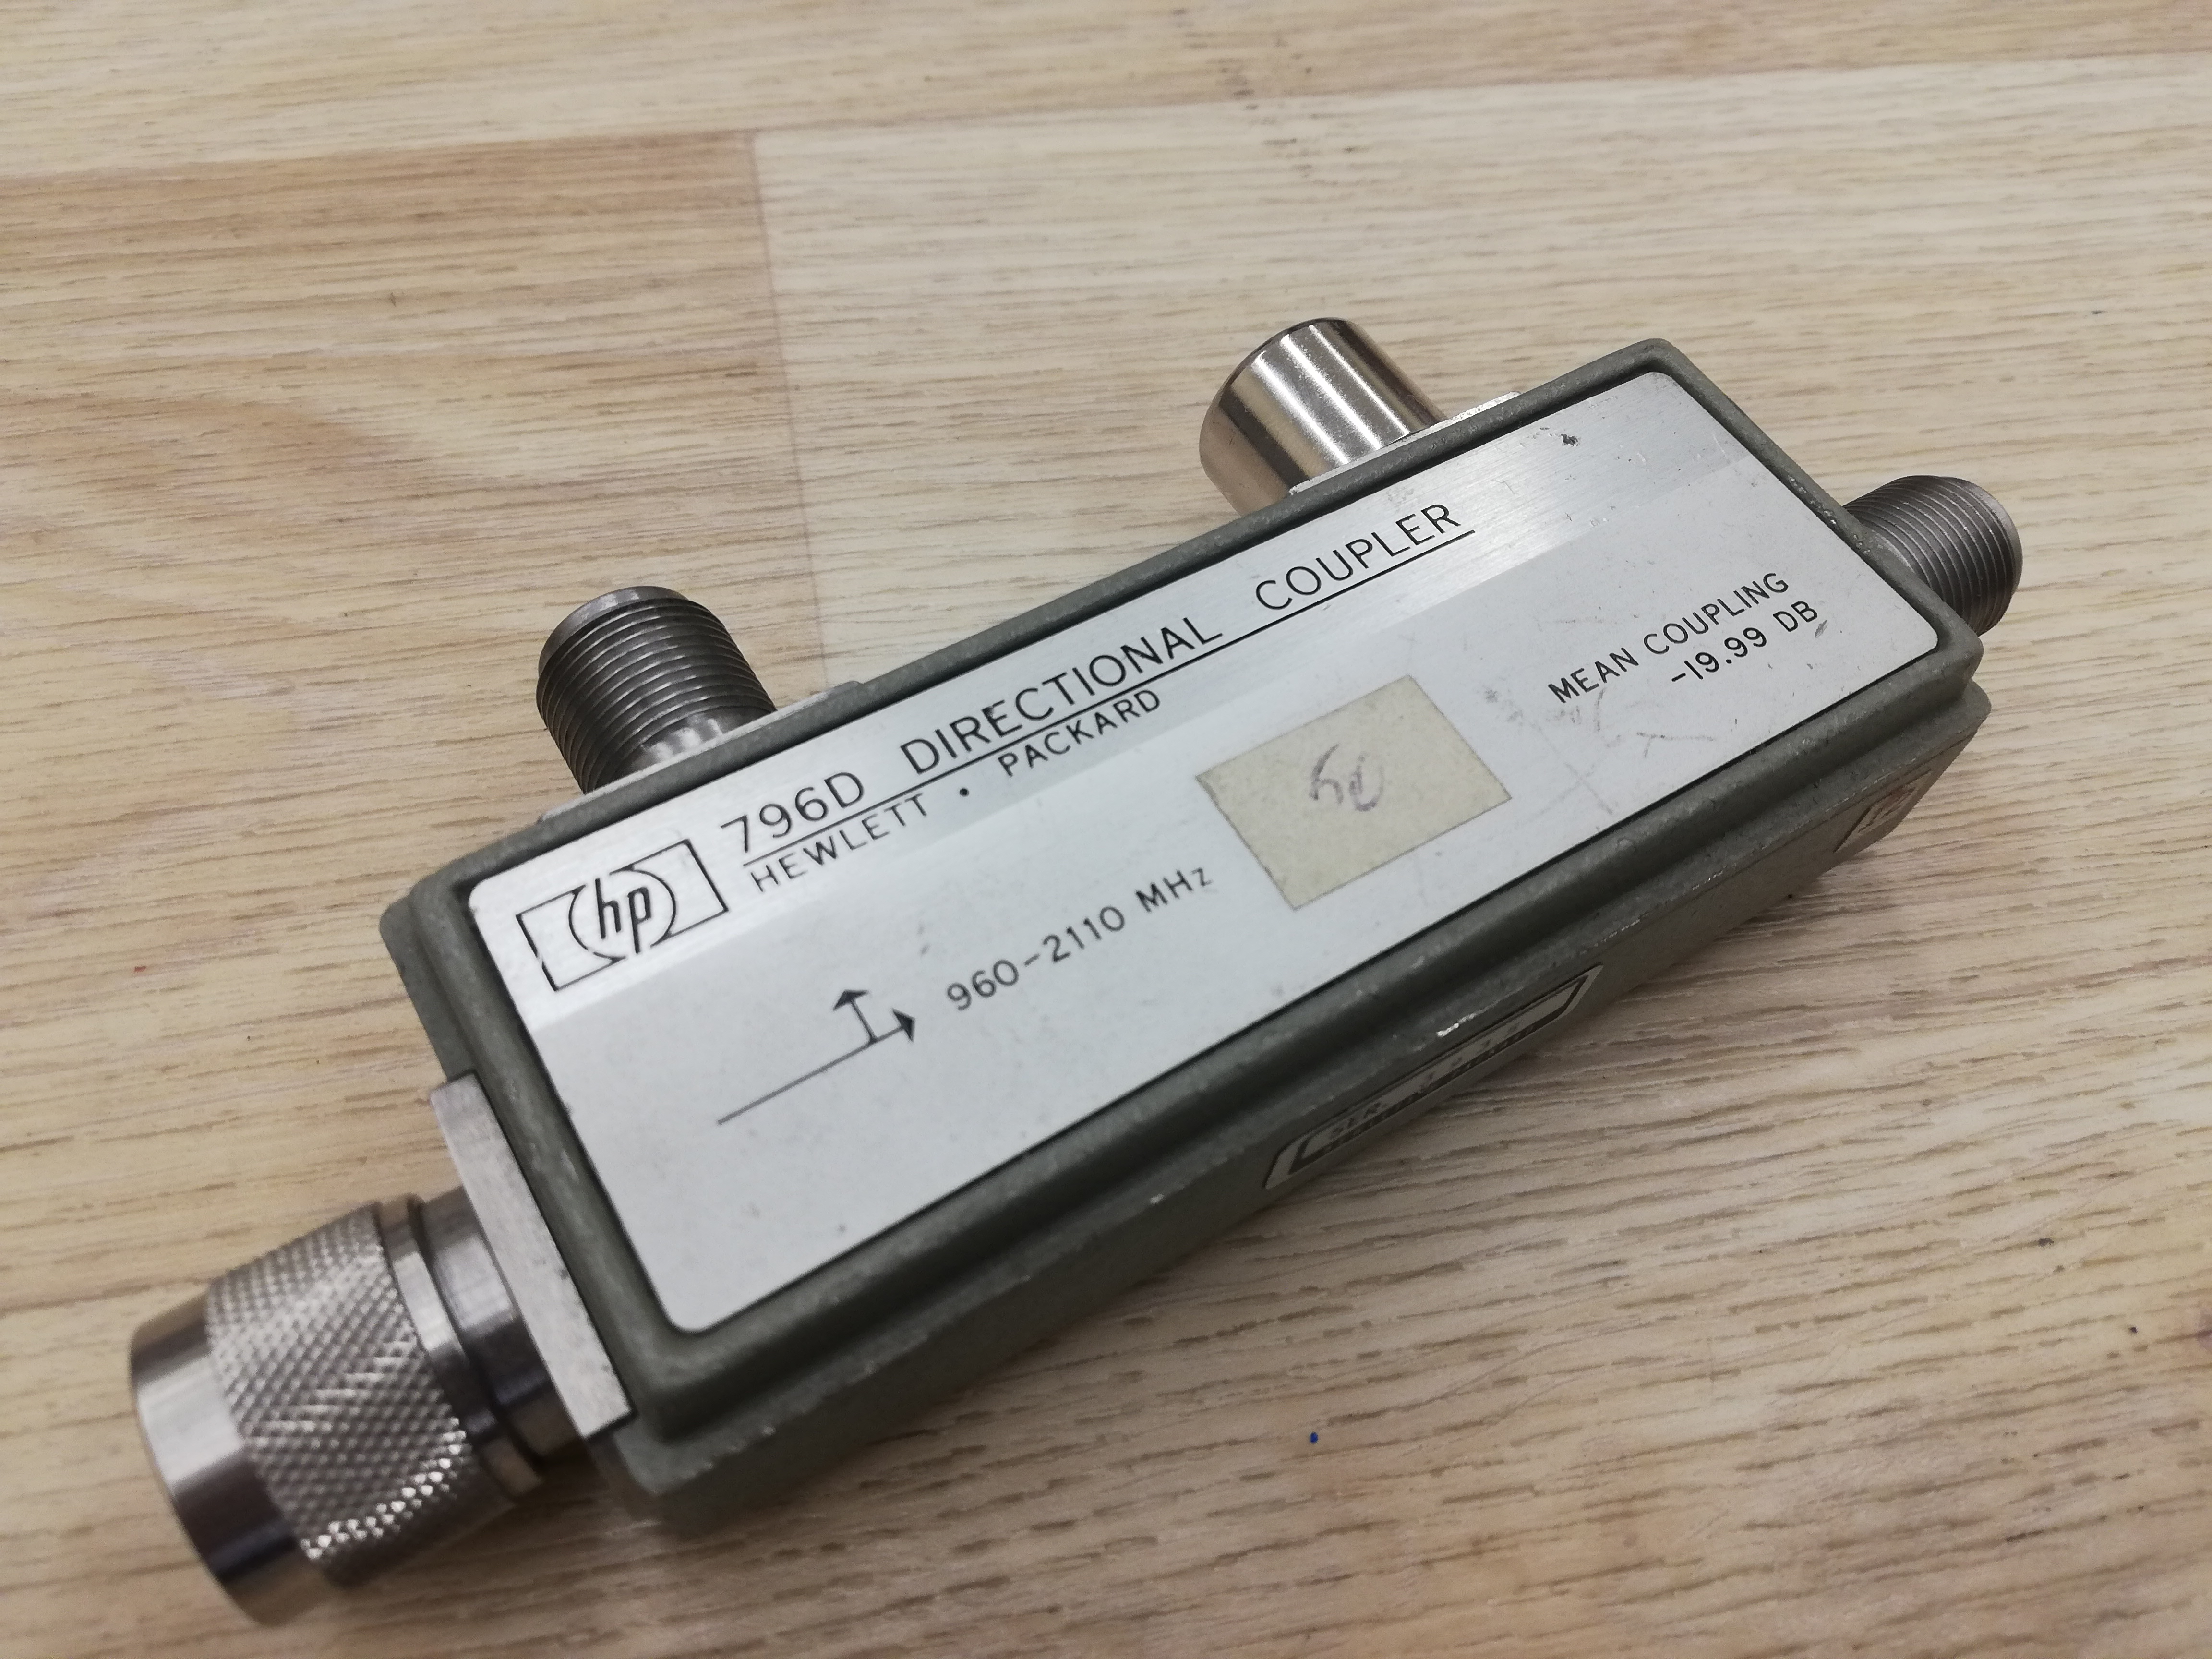
\includegraphics[width = 0.7\textwidth]{fig/796D.jpg}
        \subcaption{HP 796D.}
        \label{fig:796d}
    \end{subfigure}
    %
    \hfill
    \caption{HP usmereni sprežnjaci.}
\end{figure}

Usmereni sprežnjaci, čije su oznake modela 778D i 796D,
proizvođača \textit{Hewlett--Packard},
su prikazani na slikama \ref{fig:778d} i \ref{fig:796d}.
Usmereni sprežnjak 778D
radi u opsegu učestanosti $960$---$2110\unit{MHz}$, dok 
sprežnjak 796D radi u opsegu  $100$---$2000\unit{MHz}$.
Sprega oba sprežnjaka iznosi približno $c \approx 
20\unit{dB}$, dok su im direktivnosti 
$D \approx 30\unit{dB}$ navedene u dokumentaciji
\cite{datasheet778d, datasheet796d}. 
Važno je naglasiti da sprežnjak 778D
ima četiri pristupa čime odgovara opisu 
iz poglavlja \ref{ss:dc}, dok uređaj 796D
ima jedno ugrađeno prilagođenje na pristupu 
(3) sa slike \ref{fig:dc}, čime je pogodan
da se koristi kao uređaj $\rm DC_2$ sa slike
\ref{fig:sna_complete}.
Oba usmerena sprežnjaka su realizovana u 
mikrotrakastoj tehnici. 
%b

%
\subsubsection{Refleksioni most}
Model refleksionog mosta koji je korišćen je prikazan na slici
\ref{fig:SWR_bridge}. Ovaj usmereni sprežnjak se
realizuje kao mreža sa koncetrisanim parametrima
čija pincipska šema je prikazana na slici
\ref{fig:SWR_bridge_princ}. Performanse 
mreže dominantno ograničavaju efekti uzrokovani
feritnim simetrizatorom (balunom). 
Nominalni opseg učestanosti
u kome radi most je $0,1$--$3000\unit{MHz}$. 
Direktivnost sprežnjaka je bolja u nižem opsegu
učestanosti, kao što je prikazano i na 
karakteristici sa slike
 \ref{fig:transverters_store}. Sa te karakteristike 
 se može
 komentarisati da je ovaj model mosta primenjiv za 
 kvalitetna merenja u opsegu do oko $2,5\unit{GHz}$ i 
 za indikativna merenja dalje do $3\unit{GHz}$.
 Tehnike poboljšanja karakteristika 
 sistema opisane u \ref{ss:detektor} 
 mogu doprineti radu, posebno pri 
 primeni ovog modela usmerenog sprežnjaka.
%
\begin{figure}[ht!]
    \begin{subfigure}[b]{0.45\textwidth}
        \centering
        \includegraphics[width=0.8\textwidth]
        {fig/swr.jpg}
        \subcaption{Fotografija.}
        \label{fig:SWR_bridge}
    \end{subfigure}
    %
    %
    \begin{subfigure}[b]{0.45\textwidth}
        \centering
        \includegraphics[scale=0.9]{fig/swr_bridge.pdf}
        \subcaption{principska šema sa koncentrisanim parametrima.}
        \label{fig:SWR_bridge_princ}
    \end{subfigure}
    %
    \caption{Refleksioni most.}
\end{figure}
%
\begin{figure}[ht!]
    \centering
    \includegraphics{fig/grafik_swr.pdf}
    \caption{Direktivnost refleksionog mosta, 
    adaptirano i preuzeto iz \cite{transverters_store}.}
    \label{fig:transverters_store}
\end{figure}

Jedan od nedostataka ovog uređaja je nedostatak 
 pristupa koji izoluje talas incidentan na 
 ulaznom (\texttt{IN}) pristupu čime nije moguće 
 direktno dobiti referentni signal, što se 
 inače izvodi izdvajanjem dela pobudnog signala
 pomoću prilagođenog rezistivnog razdelnika 
 snage. Ovakva topologija sprežnjaka se koristi 
 u analizatorima mreža budući da se njegove 
 kvalitetne realizacije mogu učiniti veoma
 širokopojasnim \cite{mpk}.

\subsection{Arhitektura mernog sistema}   

Softver mernog sistema implementiran je kao 
\texttt{Python} biblioteka \texttt{ArduinoSNA} čiji kod je u celosti
dat u dodatku \ref{ap:lib}. 
Biblioteka implementira klase sa pridruženim metodoma 
koje su prikazane na slici \ref{fig:py}. Klase 
\verb|INetworkAnalyzerE5062| i \verb|IArduino| predstavljaju
interfejsne klase koje komuniciraju sa pobudnim
generatorom
i mikrokontrolerom. Klasa \verb|INetworkAnalyzerE5062| je zadužena 
za kompletnu karakterizaciju karakteristika detektora snage, 
kao i programabilni generator signala. Klasa \verb|IArduino| 
implementira dvosmernu komunikaciju za dobavljanje izmerenih
odbiraka napona na analognim ulaznim pinovima. Konačno, 
klasa \verb|Sensor| obavlja estimaciju snaga koje mere senzori 
na osnovu kalibracionih površi $\Upgamma_{\rm D}(f, P)$ 
i $V(f, P)$.
\verb||
\begin{figure}[ht!]
    \centering
    \includegraphics{fig/class.pdf}
    \caption{Pregled implementiranih klasa i metoda.}
    \label{fig:py}
\end{figure}
\subsubsection{Komunikacija sa Agilent E5062}
Komunikacija se obavlja preko LAN mreže. Računar koji pokreće merni 
sistem je konfigurisan sa statičkom IP adresom, dok je Analizatoru 
dodeljena statička IP adresa \verb|192.168.1.3|. Adresa uređaja se 
definiše u konstruktoru klase \verb|INetworkAnalyzerE5062|, 
nakon čega metoda \verb|connect()| uspostavlja vezu sa Analizatorom
koristeći se bibliotekom \verb|vxi11| \cite{vxi11}, nakon čega
se SCPI naredbama\cite{progman}
\begin{lstlisting}
CALC1:PAR1:DEF S11
CALC1:FORM MLOG
\end{lstlisting}
definiše Analizatoru da se u merenjima meri parametar $s_{11}$
u logaritamskoj skali (po magnitudi). Nakon toga analizator je
konfigurisan za dalju upotrebu. Snaga na izlazu generatora 
se postavlja metodom \verb|setPower| koja prethodno proverava 
stanje atenuatora metodom \verb|powerInBounds|, a po potrebi postavlja potrebnu vrednost atenuacije metodom \verb|setAttenuator|. Izbor
atenuatora određen je tabelom \ref{tab:att}.
\begin{table}[ht!]
    \centering
    \begin{tabular}{|c|c|} \hline
         Atenuacija [dB] & Opseg snaga [dBm]  \\ \hline \hline
         0 & $-5 \ldots 10$ \\
         10 & $-15 \ldots 0$ \\
         20 & $-25 \ldots -10$ \\
         30 & $-35 \ldots -20$ \\
         40 & $-45 \ldots -30$ \\ \hline
    \end{tabular}
    \caption{Podešavanje atenuacije.}
    \label{tab:att}
\end{table}

SCPI naredbe koje postavljaju snagu, učestanost, atenuaciju, 
centralnu učestanost i span učestanosti su
\begin{lstlisting}
SOUR1:POW <x>
SOUR1:POW:ATT <x>
SENS1:FREQ:CENT <x>
SENS1:FREQ:SPAN <x>
\end{lstlisting}
gde su \verb|<x>| vrednosti koje treba postaviti. Vrednost 
izmerenog parametra $s_{\rm 11}$, koja se doprema kao string sa 
vrednostima odvojenim zarezima, se dobija SCPI upitom oblika
\begin{lstlisting}
CALC1:DATA:FDAT?
\end{lstlisting}

\subsubsection{Komunikacija sa mikrokontorlerom}
Arduino se u ovom projektu koristi kao akvizicioni uređaj koji na
sebi ima odgovarajuće AD konvertore. Komunicira sa računarom preko
istog USB kabla kojim se napaja i programira. Na mikrokontroleru 
se koristi biblioteka \verb|Serial| za čitanje i pisanje. 
Komunikacija se obavlja brzinom (eng. \textit{baud rate}) 
od $9600\unit{bps}$. Analogni pinovi koji se koriste su 
\verb|A0|, \verb|A1| i \verb|A2|, sa kojih napone računar dobija 
slanjem upita u vidu stringova \verb|'SAMPLE0'|, \verb|'SAMPLE1'| i \verb|'SAMPLE2'| redom.
Arduino šalje napon izražen u voltima sa fizičkom rezolucijom od 
$10\unit{b}$, što približno odgovara rezoluciji po 
snazi $\Delta p \approx 20\unit{mdBm}$.

\subsubsection{Karakterizacija detektora snage
\label{ss:kds}}
Karakterizacija detektora snage se obavlja metodom tačku--po--tačku.
Snaga se menja u opsegu $[-45,\,5]\unit{dBm}$ sa korakom od 
$2,5\unit{dBm}$, dok se učestanost menja u opsegu $[1, 3]\unit{GHz}$
sa korakom $25\unit{MHz}$.
\begin{figure}[ht!]
    \centering
    \includegraphics[width=0.8\textwidth]{fig/cal_meas.png}
    \caption{Postavka karakterizacije detektora snage.}
    \label{fig:cal}
\end{figure}
Za svaku od tačaka, generatoru se šalju snaga i učestanost,
nakon čega se sa Arduina očitava izmereni napon. 
Između dva očitavanja čeka se vreme koje se definiše
pomoću metode \verb|setSafetyParams|.
Dobijeni podaci se pakuju u \verb|numpy| matricu 
čiji je format jedng reda \verb|[F, P, V, S11]|
i čuvaju kao \verb|*.npz| fajl koji se kasnije prosleđuje
pri inicijalizaciji instance senzora.

\subsubsection{Postupak izračunavanja 
rezultata merenja}

Merenje ispitivanog uređaja se radi povezivanjem
u mernu postavku sa slike \ref{fig:sna_block},
pri čemu su svi detektori snage prethodno
kalibrisani na način opisan u prethodnoj tački.
Fajlovi u kojima su opisane karakteristike 
detektora su \verb|sens|$i$\verb|_char.npz| 
($i = 1,2,3$). Kompletna skripta za izvođenje
merenja je navedena u dodatku \ref{ap:meas}. 
Merenje se obavlja tačku--po--tačku po učestanosti u opsegu
$300\unit{MHz} \leq f \leq 3\unit{GHz}$ sa korakom od $\Delta f = 10\unit{MHz}$. Važno je naglasiti da učestnost $f_0$
za koju se odrađuje merenje ne mora biti među učestanostima za koje
je rađena kalibracija. Pretpostavimo da je $f_{k} < f_0 < f_{k+1}$.
Onda se statička karakteristika detektora na učestanosti $f$ može 
proceniti na osnovu karakteristika $V(f_k, P)$ i $V(f_{k+1}, P)$,
koristeći se linearnom interpolacijom
\begin{equation}
    V_{f_0}(P) = V(f_0, P) = \dfrac{ V(f_k, P)(f_{k+1} - f_0) + 
    V(f_{k+1}, P)(f_{0} - f_k)  }{f_{k+1} - f_k}.
\end{equation}
Grafička predstava ove interpolacije je prikazana na slici
\ref{fig:interp}.
Nakon određenja odgovarajuće karakteristike, $V = V_{f_0}(P)$, 
interpolacijom odgovarajuće inverzne funckije $P = P_{f_0}(V)$
određuje se konačni rezultat incidentne snage.

\begin{figure}[ht!]
    \centering
    \includegraphics[scale=1.4
    ]{fig/3dinterp.pdf}
    \caption{Uz interpolaciju karakteristike detektora.}
    \label{fig:interp}
\end{figure}


\section{Rezultati i diskusija}
%
Obavljena su merenja postavki realizovanih
od različitih kombinacija prethodno opisanih 
uređaja, a u cilju ilustracije izvedenih relacija. 
Formirane su dve merne konfiguracije:
\begin{enumerate}[(K1)]
    \item Profesionalni usmereni sprežnjaci, 
    sa i bez atenuatora na 
    detektorima, prikazana na slici 
    \ref{fig:setup1}
    \item Refleksioni most na ulazu, sa i bez atenuatora
    na detektorima, prikazana na slici 
    \ref{fig:setup2}
\end{enumerate}
%
\begin{figure}[ht!]
    \begin{subfigure}[b]{0.49\textwidth}
        \centering
        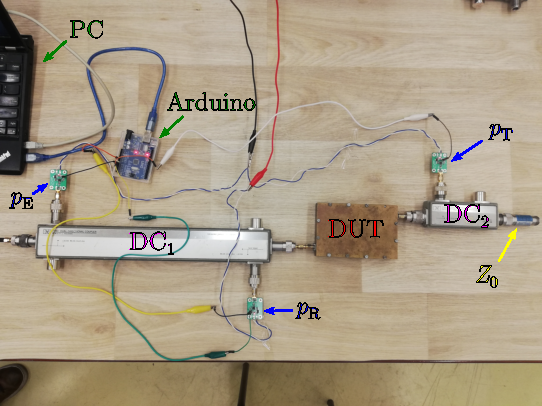
\includegraphics[width = 1\textwidth]{fig/setup1.png}
        \subcaption{Postavka (1).}
        \label{fig:setup1}
    \end{subfigure}
    \hfill
    \begin{subfigure}[b]{0.49\textwidth}
        \centering
        \includegraphics[width = 1\textwidth]{fig/setup2.png}
        \subcaption{Postavka (2).}
        \label{fig:setup2}
    \end{subfigure}
    %
    \caption{Fotografije mernih postavki.}
\end{figure}
%
\begin{figure}[ht!]
    \begin{subfigure}[b]{0.49\textwidth}
        \centering
        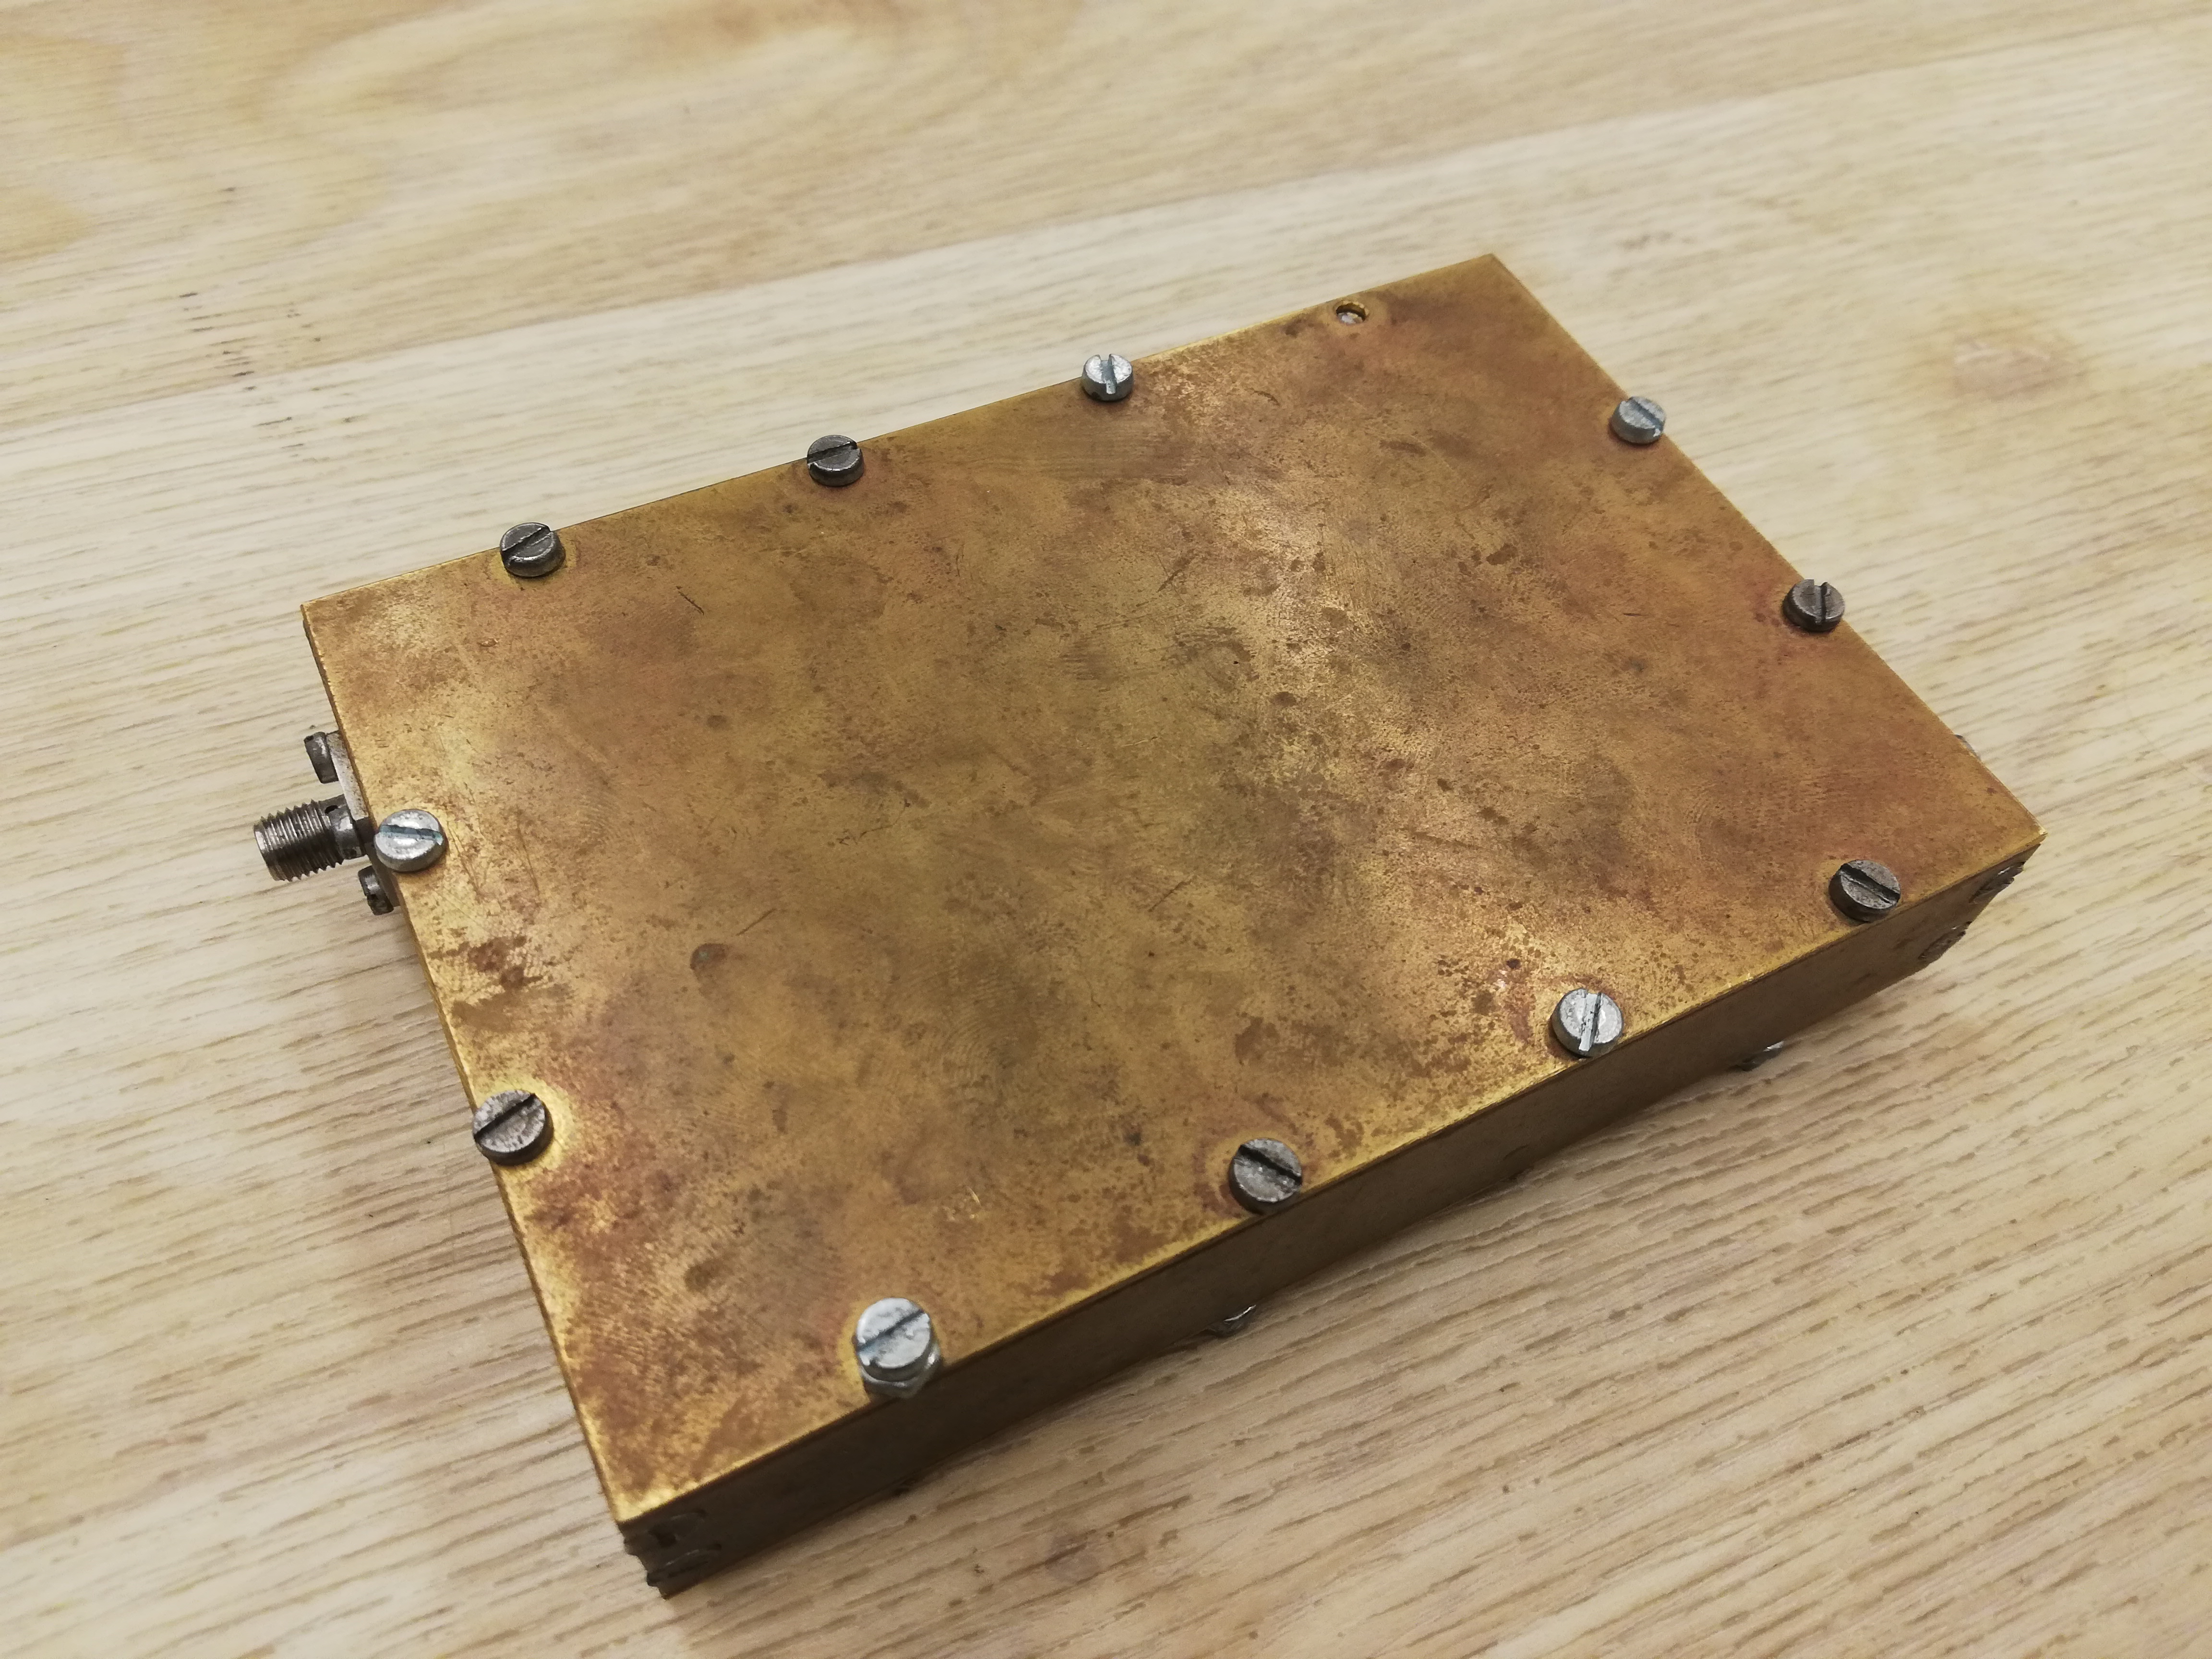
\includegraphics[width = 1\textwidth]{fig/bpf.jpg}
        \subcaption{Filtar propusnik opsega učestanosti.
         }
        \label{fig:bpf}
    \end{subfigure}
    \hfill
    \begin{subfigure}[b]{0.49\textwidth}
        \centering
        \includegraphics[width = 1\textwidth]{fig/att.jpg}
        \subcaption{Atenuator.
         }
        \label{fig:att}
    \end{subfigure}
    %
    \caption{Fotografije ispitivanih mreža.}
\end{figure}
%
Merenja su obavljena za dva uređaja koji su:
\begin{enumerate}[(U1)]
    \item 
Filtar propusnik opsega učestanosti, 
čija je centralna učestanost
oko $1,8\unit{GHz}$, koji ima pristupe sa ženskim SMA konektorima,
prikazan na slici \ref{fig:bpf}
\item Atenuator slabljenja 
$10\unit{dB}$, čiji je propusni opseg do 
$12\unit{GHz}$, proizvođača 
\textit{Hewlett--Packard}, koji ima N konektore, prikazan
na slici \ref{fig:att}. 
\end{enumerate}
Prelazi sa  
N konektora na SMA konektore i obratno će se u nastavku,
za potrebe ovog rada, smatrati savršenim. U 
svim ogledima snaga pobudnog generatora 
je podešena na vrednost $10\unit{dBm}$.
%
\subsection{Ogledi}

\subsubsection{Ogled 1}
Mereni su parametri rasejanja uređaja (U1) 
konfiguracijom (K1) bez upotrebe atenuatora ispred
detektora snage. Rezultati su upoređeni sa 
referentnim merenjem sa Analizatora mreža 
na slici \ref{fig:ogled1}. Rezultati pokazuju 
dobro poklapanje sa referentnim instrumentom.
%
\begin{figure}[ht!]
    \begin{subfigure}[b]{0.49\textwidth}
        \centering
        \includegraphics[width = 1\textwidth]{fig/s11_bpf.png}
        \subcaption{Rezultati merenja 
        refleksije na ulaznom pristupu.}
        \label{fig:s11_bpf}
    \end{subfigure}
    \hfill
    \begin{subfigure}[b]{0.49\textwidth}
        \centering
        \includegraphics[width = 1\textwidth]{fig/s21_bpf.png}
        \subcaption{Poređenje rezultata merenja sa referentnim
        insturmentom.}
        \label{fig:s21_bpf}
    \end{subfigure}
    %
    \caption{Uz ogled 1.}
    \label{fig:ogled1}
\end{figure}
%
Prag osetljivosti određen je minimalnom snagom
koju detektori snage mogu pouzdano da mere, koja
iznosi približno $-60\unit{dBm}$, što se 
jasno i vidi u dobijenim rezultatima. Činjenica da 
je poklapanje sa referenetnim instrumentom dobro
sve do praga osetljivosti detektora ukazuje na
to da je ograničavajući faktor osetljivost 
detektora, a ne prilagođenja u mreži, usled čega 
se performanse ove konfiguracije ne mogu značajno
unaprediti dodavanjem atenuatora.

\subsubsection{Ogled 2}
Mereni su parametri rasejanja uređaja (U1) 
konfiguracijom (K1) sa i bez upotrebe atenuatora  
od $10\unit{dB}$
ispred detektora snage, a
dobijeni rezultati su
prikazani na slici \ref{fig:ogled2}. Kao
što je komentarisano u rezultatu ogleda 1, 
dodavanje atenuatora ne doprinosi funkciji 
ove konfiguracije. 
Brz propad karakteristike nakon učestnosti oko 
$2\unit{GHz}$ se može objasniti tehnikom 
izrade sprežnjaka.

\begin{figure}[ht!]
    \begin{subfigure}[b]{0.49\textwidth}
        \centering
        \includegraphics[width = 1\textwidth]{fig/s11_att.png}
        \subcaption{Merenja parametra refleksije.}
        \label{fig:s11_att}
    \end{subfigure}
    %
    \begin{subfigure}[b]{0.49\textwidth}
        \centering
        \includegraphics[width = 1\textwidth]{fig/s21_att.png}
        \subcaption{Merenja parametra transmisije.}
        \label{fig:s21_att}
    \end{subfigure}  
    %
    \caption{Uz ogled 2.}
    \label{fig:ogled2}
\end{figure}

\subsubsection{Ogled 3}
Mereni su parametri rasejanja uređaja (U1) 
konfiguracijom (K2) sa i bez upotrebe atenuatora  
ispred detektora reflektovanog nivoa snage
$A_{\rm R} = 10\unit{dB}$, a dobijeni rezultati 
prikazani su na slici \ref{fig:ogled3}. 
Budući da ova konfiguracija nema referentno
merenje, nacrtana je izmerena snaga reflektovanog
talasa. Važno je posebno naglasiti da se 
uticaj atenuatora kvalitativno razlikuje u 
slučaju željenog signala i u slučaju izobličenja
uzrkovanih nesavršenošću instrumenta, što se 
može videti na slici \ref{fig:pR_bpf}. To se 
posebno može uočiti na višim učestanostima 
gde je neprilagođenje detektora loše. 
U pogledu merenja transmitovane snage,
sa slike \ref{fig:pT_bpf}, očekivano se ne uočava
značajan doprinos dodatnog atenuatora.

\begin{figure}
    \begin{subfigure}[b]{0.49\textwidth}
        \centering
        \includegraphics[width = 1\textwidth]{fig/pR_bpf.png}
        \subcaption{Merenje nivoa 
        reflektovane snage.}
        \label{fig:pR_bpf}
    \end{subfigure}
    %
    \begin{subfigure}[b]{0.49\textwidth}
        \centering
        \includegraphics[width = 1\textwidth]{fig/pT_bpf.png}
        \subcaption{Merenja nivoa 
        transmitovane snage.}
        \label{fig:pT_bpf}
    \end{subfigure}  
    %
    \caption{Uz ogled 3.}
    \label{fig:ogled3}
\end{figure}

\subsubsection{Ogled 4}
%
\begin{figure}[b!]
    \centering
    \includegraphics{fig/pR_bpf2.png}
    \caption{Uz ogled 4.}
    \label{fig:ogled4}
\end{figure}
%
Mereni su parametri rasejanja uređaja (U1) 
konfiguracijom (K2), povećavajući vrednost
atenuacije u odnosu na prethodnu tačku na
$A_{\rm R} = 40\unit{dB}$. Rezultati merenja 
refleksije prikazani su na slici 
\ref{fig:ogled4}. Odsecanje signala  
uzrokovano je osetljivošću senzora budući
da je taj nivo podignut za atenuaciju 
radi diskusije. Može se primetiti da se 
oblik smetnji u okolini učestanosti 
$2,5\unit{GHz}$ nije značajno potisnuo
povećanjem atenuacije do $40\unit{dB}$. 
U ovom ugledu, uticaj atenuacije je kvalitativno drugačiji
u odnosu na pređašjni ogled. Nije 
ustanovljena kvalitativna razlika između dejstva 
na signal i na smetnju odakle se može tvrditi da 
je slabljenje od $10 \unit{dB}$ zaista blizu optimalnog
što je u skladu sa rezultatom iz jednačine (14), 
imajući u vidu 
da je na osnovu osnovu grafika sa slike
\ref{fig:transverters_store}, direktivnost usmerenog
sprežnjaka $D(2,5\unit{GHz}) \approx 
20\unit{dB}$.

\subsection{Diskusija i zaključak}
U ovom radu je izložen opšti postupak projektovanja 
skalarnog analizatora mreža polazeći od pristupačnih uređaja
i njihovom integracijom u kompletan sistem. Tom prilikom je u
odeljku \ref{ss:detektor}
izvedena veza za optimalno slabljenje atenuatora za prilagođenje
detektora snage, koja je i dokazana na osnovu rezultata ogleda 3 i 4. 
Na osnovu rezultata ogleda 1 se može tvrditi da su postupak kalibracije
detektora snage, kao i kompletan \textit{end-to-end} sistem ispravni 
i funkcionišu u skladu sa očekivanjima. Takođe treba da naglasiti
da je opseg učestanosti $300\unit{MHz}$---$3\unit{GHz}$ određen prvenstveno
karakteristikama upotrebljenog izvora signala, te da se on može proširiti
koristeći se sličnim komponentama, a zadržavajući istu metodologiju
projektovanja. 

Na osnovu rezultata izvedenih ogleda, a imajući u vidu 
teorijske rezultate navedene u odeljku 3, može se zaključiti
da načelno obe ispitane konfiguracije funkcionišu u skladu
sa očekivanjima.

Implementirana biblioteka u ovom radu se može iskorstiti 
i za softversku podršku za naprednije sisteme, budući 
da su korišćeni protokoli standardizovani i praktično 
isti nad raznim uređajima raznih proizvođača. Specifičnosti 
bi se u tom pogledu odnosile pre svega na rečnik 
naredbi koji za svaki instrument može biti
specificiran, ali je naveden u odgovarajućem 
uputstvu za programere (eng. \textit{Programmers' manual}). 

Dalji rad na ovom projektu mogao bi se odnositi
na kvalitetniju realizaciju mreža za prilagođenje
detektora snage, čime bi se ostvario 
širi opseg učestanosti u kome je njegovo 
prilagođenje prihvatljivo. Takođe, potrebno 
je ispitati rad sistema sa pristupačnijim
programabilnim generatorima signala, koji 
eventualno rade u širem opsegu učestanosti.


\begin{thebibliography}{9}

\bibitem{Peja1}
P. Pejović, „Princip rada i primena osciloskopa“, Beograd 2016,  
dostupno na \url{https://zenodo.org/record/1311555#.X0QuahFS8pg}, 
poslednji put pristupljeno \today

\bibitem{mwmeas}
R. J. Collier and A. D. Skinner, „Microwave Measurements 3rd Edition“, The Institution of Engineering and Technology, 2007.

\bibitem{djordjevic-mw}
A. Đorđević, D. Tošić, „Mikrotalasna tehnika“, 1. izdanje, Akademska misao, Beograd, 2006. 

\bibitem{pozar}
D. Pozar, „Microwave Engineering“, J. Wiley, New York, 2012.

\bibitem{transverters_store}
\textit{Transverters-Store, RF bridge}, dostupno na
\url{https://transverters-store.com/rf_bridge/rf_bridge.html}

\bibitem{datasheet778d}
Proizvođačka dokumentacija 
\textit{Hewlett Packard} 778D, dostupna na
\url{http://literature.cdn.keysight.com/litweb/pdf/5952-8133.pdf},
poslednji put pristupljeno \today

\bibitem{datasheet796d}
Proizvođačka dokumentacija, 
\textit{Hewlett Packard} 796D, dostupna na
\url{https://testequipment.center/Product_Documents/Agilent-796D-Specifications-99658.pdf},
poslednji put pristupljeno \today

\bibitem{mpk}
V. Petrović, D. Tošić, A. Đorđević 
„Mikrotalasna pasivna kola“, Beograd, 2010, slobodno
dostupano na
\url{https://www.etf.bg.ac.rs/uploads/files/udzbenici/MPK_2010.pdf}, 
poslednji put pristupljeno \today

\bibitem{ad8318}
Proizvođačka dokumentacija 
\textit{Analog Devices} AD8318, dostupna na
\url{https://www.analog.com/media/en/technical-documentation/data-sheets/ad8318.pdf},
poslednji put pristupljeno \today

\bibitem{vxi11}
\verb|Python| paket \verb|vxi11|, dostupno
na \url{https://pypi.org/project/python-vxi11/},
poslednju put pristupljeno \today

\bibitem{progman}
\textit{Agilent E5061A/E5062A ENA SeriesENA Series RF Network Analyzers Programmer’s Guide},
dostupno na \url{http://literature.cdn.keysight.com/litweb/pdf/E5061-90042.pdf}, poslednji 
put pristupljeno \today

\end{thebibliography}



\newpage
\appendix
\chapter*{Dodatak}
\addcontentsline{toc}{chapter}{Dodatak}

\section{K\^od implementirane biblioteke \label{ap:lib}}
\input{arduinosna_py}


\section{Skripta za prikupljanje merenja \label{ap:meas}}
\begin{lstlisting}[language=Python]

from pylab import np, plt
from arduinosna import *

NA = INetworkAnalyzerE5062('192.168.1.3')
NA.setSafetyParams(delay = 0.2, Pmax = 5, Pmin = -45)
NA.connect()

ARD = IArduino(dev = '/dev/ttyUSB0', baudRate = 9600, timeout = 2.00)
ARD.setSafetyDelay(0.1)
ARD.connect()

# Input - power
freq_v = np.arange( 900e6, 3e9, 10e6 )
print (freq_v)

# Output - measurements
V0_vector = np.zeros(np.size(freq_v))
V1_vector = np.zeros(np.size(freq_v))
V2_vector = np.zeros(np.size(freq_v))
S11_vector = np.zeros(np.size(freq_v))

j = 0

for f in freq_v:
    NA.setFrequency(f)
    ARD.command("SAMPLE0")
    V0_vector[j] = ARD.read()

    ARD.command("SAMPLE1")
    V1_vector[j] = ARD.read()

    ARD.command("SAMPLE2")
    V2_vector[j] = ARD.read()

    j+=1

np.savez("Filtar_Characteristics_2.npz", 
         f = freq_v, V0 = V0_vector, V1 = V1_vector, V2 = V2_vector)
\end{lstlisting}

\newpage
\section{Skripta za obradu rezultata merenja \label{ap:orm}}

\begin{lstlisting}[language=Python]
d = np.load("Filtar_Characteristics_2.npz")
f = d["f"]
V0 = d["V0"]
V1 = d["V1"]
V2 = d["V2"]

R_sens = Sensor("data/sens1_char.npz")
E_sens = Sensor("data/sens2_char.npz")
T_sens = Sensor("data/sens3_char.npz")

_, PR = R_sens.measure(f, V0)
_, PE = E_sens.measure(f, V2)
_, PT = T_sens.measure(f, V1)

plt,figure(1)
plt.plot(f/1e9, PR)
plt.plot(f/1e9, PE)
plt.plot(f/1e9, PT)
legend(["R", "E", "T"])
plt.xlabel(u"$f$ [GHz]")
plt.ylabel(u"$P$ [dBm]")
plt.grid()

S21 = PT-PE
S11 = PR-PE # Odredjivanje S parametara

## Extract refference value
ref_data = np.genfromtxt('../S21.CSV', delimiter=',', skip_header=3)
print(ref_data[:][0]/1e9)

plt.figure(2)
plt.plot(f/1e9, S21)
plt.plot(f/1e9, S21)
plt.xlabel(u"f [GHz]")
plt.ylabel(r"$S_{21}$, $S_{11}$ [dB]")
plt.grid()

plt.show()
\end{lstlisting}


%
\end{document}